

%\documentclass{article}
%\documentclass[12pt,twoside,openright]{report} - with white page between major sections
\documentclass[12pt]{report}

%% Useful packages
\usepackage[a4paper,top=1in,bottom=1in,left=1in,right=1in]{geometry}
\usepackage{amsmath, amssymb, bm}
\usepackage{caption}
\usepackage{graphicx}
\usepackage[colorinlistoftodos]{todonotes}
\usepackage[colorlinks=true, allcolors=black]{hyperref}
\usepackage{float}
\usepackage{setspace}
\usepackage{subfigure}
\usepackage{url}
\usepackage{tabularx}
\usepackage[utf8]{inputenc}
\usepackage{mathptmx} %Times Font
\usepackage{titlesec}
\titlespacing{\chapter}{0pt}{0pt}{0pt}
\usepackage{fancyhdr}
\usepackage{etoolbox}
\usepackage{appendix}
\usepackage{siunitx}
\usepackage{nomencl}
\newcommand{\nomunit}[1]{%
\renewcommand{\nomentryend}{\hspace*{\fill}#1}}
\makenomenclature
\usepackage{caption}
\usepackage{lipsum}
\usepackage{algpseudocode}
\usepackage{empheq}
\usepackage{mdwlist}
\usepackage{booktabs}
\usepackage{colortbl}
\widowpenalty 10000
\clubpenalty 10000
\usepackage{moresize}
\usepackage{adjustbox}

\usepackage[backend=biber, style=numeric]{biblatex}
\addbibresource{References.bib}
\DeclareSourcemap{
  \maps[datatype=bibtex]{
    \map{
       \step[fieldsource=title, match=\regexp{\b([A-Z]{2,})\b}, replace={{}{$1}}]
    }
  }
}

\captionsetup[figure]{skip=15pt}
 


\DeclareCaptionType{appfigure}[Figure]
\DeclareCaptionType{apptable}[Table]
\renewcommand{\listappfigurename}{List of Appendix Figures}
\renewcommand{\listapptablename}{List of Appendix Tables}
\renewcommand{\thefigure}{\thechapter-\arabic{figure}}
\renewcommand{\thetable}{\thechapter-\arabic{table}}
\renewcommand{\theappfigure}{\thechapter-\arabic{appfigure}}
\renewcommand{\theapptable}{\thechapter-\arabic{apptable}}
\renewcommand{\contentsname}{Table of Contents}

\newcommand{\chapname}{Chapter }
 
\titleformat{\chapter}[block]
{\bfseries\LARGE\centering}
{}{1em}{}[\rule{\textwidth}{0.3pt}]

\titleformat{\section}
{\bfseries\large}
{\thesection}{1em}{}

\titleformat{\subsection}
{\normalfont\bfseries}
{\thesubsection}{1em}{}

\titleformat{\subsubsection}
{\normalfont\bfseries}
{\thesubsubsection}{1em}{}

\usepackage{fancyhdr}
\usepackage{multirow}
\usepackage{multicol}

\usepackage{placeins}

\makeatletter
\renewcommand*\env@matrix[1][*\c@MaxMatrixCols c]{%
  \hskip -\arraycolsep
  \let\@ifnextchar\new@ifnextchar
  \array{#1}}
\makeatother

\usepackage{enumitem}

\usepackage{listings}
\usepackage{color}
 
\definecolor{codegreen}{rgb}{0,0.6,0}
\definecolor{codegray}{rgb}{0.5,0.5,0.5}
\definecolor{codepurple}{rgb}{0.58,0,0.82}
\definecolor{backcolour}{rgb}{0.95,0.95,0.95}

\newcommand{\codesize}{\fontsize{10pt}{11pt}\selectfont}

\lstdefinestyle{mystyle}{
    backgroundcolor=\color{backcolour},   
    commentstyle=\color{codegreen},
    keywordstyle=\color{magenta},
    numberstyle=\tiny\color{codegray},
    stringstyle=\color{codepurple},
    basicstyle=\ttfamily\codesize,
    breakatwhitespace=true,         
    breaklines=true,                 
    captionpos=b,                    
    keepspaces=false,                 
    numbers=left,                    
    numbersep=5pt,                  
    showspaces=false,                
    showstringspaces=false,
    showtabs=false,                  
    tabsize=2,
    showlines = true,
    fontadjust = true,
    framexleftmargin = 10 pt,
    resetmargins = true,
    basewidth = 0.5em
}
\setlength{\parskip}{1em} % Adjust '1em' to your desired space
\setlength{\floatsep}{20pt}    % Space between figures/tables (float objects)
\setlength{\textfloatsep}{20pt} % Space between figures and text
\setlength{\intextsep}{20pt}    % Space above/below inline figures and text
\lstset{style=mystyle}

\makeatletter
\setlength{\@fptop}{0pt}
\makeatother

\setlength{\floatsep}{0pt}

\newenvironment{Figure}
  {\noindent\minipage{\linewidth}}
  {\endminipage}

\setcounter{secnumdepth}{5}

\hyphenpenalty 10000
\usepackage{multicol}
 
%%%%%%%%% MATHEMATICS SHORTHANDS %%%%%%%%%%%%%%%%%%%% 

\newcommand{\C}{\mathbb{C}}
\newcommand{\R}{\mathbb{R}}
\newcommand{\Z}{\mathbb{Z}}
\renewcommand{\d}{\mathrm{d}}
\renewcommand{\bf}[1]{\mathbf{#1}}

\newcommand{\argmax}[1]{\underset {#1}{\operatorname{arg\,max}}}

\newcommand{\kurt}{\mathrm{kurt}}
\newcommand{\round}{\operatorname{round}}

\newcommand{\E}{\operatorname{E}}
\newcommand{\cov}{\operatorname{cov}}
\newcommand{\pcov}{\operatorname{pcov}}

\newcommand*{\vertbar}{\rule[-1ex]{0.5pt}{2.5ex}}
\newcommand*{\horzbar}{\rule[.5ex]{2.5ex}{0.5pt}}

\setlength{\nomlabelwidth}{3cm}
\setlength{\nomitemsep}{-0.5\parsep}

\usepackage{makecell}
\usepackage{emptypage}

\newcolumntype{R}{>{\raggedleft\arraybackslash}X}
\newcolumntype{L}{>{\raggedright\arraybackslash}X}
\newcolumntype{C}{>{\centering\arraybackslash}X}

\usepackage{textcomp}

%
%\usepackage{background}

%\SetBgScale{1}
%\SetBgContents{\parbox{10cm}{%
%  \Huge Draft:  \today\\[14cm]\rotatebox{180}{\Huge Draft:  %\today}}}
%\SetBgColor{gray}
%\SetBgAngle{270}
%\SetBgOpacity{0.1}
%

%%%%%%%%%%%%%%%%%%%%%%%%%%%%%%%%%%%%%%%%%%%%%%%%%%%%%
\begin{document}
\sloppy
%==== FRONT PART====
\begin{titlepage}
\begin{figure}[!t]
\centering

\includegraphics[width = 4.2in]{Title/logo.png}
\caption*{}
\end{figure}

\centering
\LARGE{\textbf{Infrastructure Provisioning for SpeechLab Applications with Terraform}}\\[1in]

\LARGE{\textbf{Chan Ming Han}}\\
\vspace{0.2in}
\normalsize{U2120477J}\\[0.2in]

\large{Supervisor: Prof Chng Eng Siong}\\
% \large{Co-supervisor: XXXXX}\\[0.5in]
\vspace{0.2in}

\large{A Final Year Report submitted to School of Computer Science and Engineering, Nanyang Technological University in partial fulfilment of the requirements for the Degree of }\\[0.1in]

\Large{BACHELOR OF ENGINEERING SCIENCE (COMPUTER ENGINEERING)
}\\[1in]


\Large{2024/2025 Semester 2}
\newpage
\end{titlepage}

%\begingroup
%\let\cleardoublepage\clearpage
\pagenumbering{roman}
\pagestyle{fancy}
\fancyhf{}
\cfoot{\thepage}
%\endgroup

%=== FRONT PART ===
%=== ABSTRCT ===

%\begin{center}
\chapter*{Abstract}
\rhead{Abstract}
%\end{center}
\addcontentsline{toc}{chapter}{Abstract}
%===============================
% ABSTRACT GOES HERE - 250 words limit
%===============================
As companies move toward containerisation technologies to improve scalability and portability in their applications, Kubernetes has emerged as the industry standard for orchestrating containerised workloads. Despite its advantages, deploying containerised workloads to the cloud is highly complex, and resource intensive. Developers and engineer also need to master the various cloud technologies, such as security and networking requirements, often diverting focus from core application development. 
This project introduces cloudkube, a lightweight, Python-based command-line tool designed to automate the deployment of Kubernetes clusters in the cloud. Inspired by minikube and leveraging Infrastructure as Code (IaC) principles with Terraform, cloudkube abstracts the complexities of cloud provisioning and Kubernetes setup. It enables developers to focus on core application development, rather than cloud or deployment configurations.. The tool supports customizable configurations, automated local environment setup, and idempotent resource provisioning while ensuring low-cost prototyping by leveraging AWS Free Tier resources.
Through cloudkube, deployment times are significantly reduced, and infrastructure provisioning is made accessible to users without deep expertise in cloud technologies. This paper details the tool’s architecture, implementation, and workflow, showcasing its potential to enhance productivity, reduce operational overhead, and accelerate the deployment of containerised applications to the cloud. 
%===============================
\\
\par
\textbf{Keywords:} Containerization, Cloud Automation, Infrastructure as Code (IaC), Terraform, Cloud Deployment, Kubernetes Orchestration, Developer Productivity, Lightweight CLI Tools, Cloud-Native Applications

%=== END OF ABSTRACT ===

\newpage

% \include{Front/Graphical_Abstract}
% \newpage

%=== FRONT PART ===
%=== ACKNOWLEDGEMENT ===

%\begin{center}
\chapter*{Acknowledgement}
\rhead{Acknowledgement}
%\end{center}
\addcontentsline{toc}{chapter}{Acknowledgement}

I would like to express my deepest gratitude to my academic advisors and mentors, including but not limited to Prof Chng Eng Siong, Research Assistant Vu Thy Ly, and James. Their guidance and invaluable insights have been instrumental throughout the course of this project. Their continuous support and constructive feedback have greatly enhanced the quality of my work. I am particularly grateful for their encouragement and inspiration, which motivated me to tackle complex challenges and explore innovative solutions.

I extend my sincere thanks to my peers, who contributed through stimulating discussions and innovative ideas. Their willingness to share knowledge and exchange ideas fostered an enriching environment that enabled the successful completion of this project.

Finally, I would like to acknowledge the funding and infrastructure support provided by Nanyang Technological University. The access to the AWS cloud platform significantly facilitated the implementation and testing phases of this project. Without their generous support, this work would not have been possible.









%=== END OF ACKNOWLEDGEMENT  ===

\newpage
\setcounter{tocdepth}{2}

\tableofcontents
\rhead{Table of Contents}
\newpage

%\include{Front/Nomenclature}
%\newpage

\renewcommand{\listfigurename}{Lists of Figures}
\rhead{Lists of Figures}
\listoffigures 
\addcontentsline{toc}{chapter}{Lists of Figures}

\newpage


\listoftables 
\addcontentsline{toc}{chapter}{Lists of Tables}
\rhead{Lists of Tables}
\newpage

\rhead{}
\setlength{\parindent}{0pt}

%==== MAIN PART ====
\clearpage
\pagenumbering{arabic} % Restart numbering in Arabic numerals
\setcounter{page}{1}   % Reset page number to 1
\chapter{Chapter 1: Introduction}
\section{Background}
In recent years, Kubernetes has emerged as the de facto standard for container orchestration, revolutionizing the way modern applications are deployed and managed \cite{google-no-date}. 
Organizations are incresingly adopting containerized workloads to leverage their multiple benefits, including scalability, portability, and efficiency in managing microservices architectures.
Kubernetes provides a robust framework for orchestrating these workloads, ensuring automated deployment, scaling, and operation of such workloads in a highly resilient manner. 

Despite the myriad of benefits that Kubernetes offers, the setup, and management of a Kubernetes cluster can often be complex and extremely time-consuming. The deployment
process involves provisioning infrastructure, configuring networking, setting up security rules, and configuring various add-ons, all of which require expertise and manual effort. For 
organizations and developers looking to ship quickly, this complexity introduces delays in application deployment, and reduces team velocity.

The traditional approach to deploying a containerised application and provisioning Kubernetes clusters in the cloud often involves multiple steps, including managing cloud provider integrations, and 
a lot of configuration. This process can take hours, or even days, depending on the use case, and the specific configuration required. As businesses demand quicker iteration cycles and seamless
cloud integration, there is a growing need for simplified, automated provisioning solutions that reduce setup time and eliminate operational friction.

As such, for this final year project, I have decided to build \texttt{cloudkube}, which steamlines the provisioning of Kubernetes clusters in the cloud, enabling users to spin up fully
configured clusters in the cloud within minutes. By abstracting away the complexities of infrastructure management, \texttt{cloudkube} allows developers to focus on deploying applications rather 
than managing the underlying infrastructure. This report explores the design, implementation, and impact of \texttt{cloudkube} in accelerating Kubernetes adoption while maintaining the flexibility
and robustness required for production grade deployments.




\section{Objective}
The main objective of this project was to speed up the turnaround time for deployment of new SpeechLab applications. The main idea of this tool is to abstract away in-depth knowledge of cloud technologies from researchers, and allow them to readily and easily deploy their ASR applications to the cloud at the press of a button. This will allow researchers to then concentrate their efforts on the development of the ML model in the ASR application, and not have to worry about low-level cloud implementation details such as creating a security group role to allow ingress/egress traffic, or configuring their local environment to hit the cluster.  

Drawing inspiration from minikube, which is a quick way to spin up a local cluster, for this FYP, I have decided to build \texttt{cloudkube}, which quickly spins up a Kubernetes cluster in the  cloud. Users then have a simple barebones Kubernetes cluster hosted in the cloud where they can do dev testing. 

The functional requirements for this project are detailed as follows:
\vspace{-1em} % Adjust vertical space here
\begin{enumerate}[label=\alph*., itemsep=0pt]
    \item \texttt{cloudkube} should provision infrastructure such as compute instances, storage, networking, and Kubernetes clusters in the cloud.
    \item \texttt{cloudkube} should be easily extendable to different cloud providers.
    \item \texttt{cloudkube} should create a Kubernetes environment, including deploying essential components like ingress controllers.
    \item \texttt{cloudkube} should allow users to easily deploy containerized ASR applications to the Kubernetes cluster.
    \item \texttt{cloudkube} should be able to deprovision and clean up resources without leaving anything dangling to prevent unnecessary costs.
    \item \texttt{cloudkube} should maintain the state of provisioned infrastructure to avoid dangling resources in the cloud.
\end{enumerate}
The non-functional requirements for this project are detailed as follows:
\vspace{-1em} % Adjust vertical space as needed

\begin{enumerate}[label=\alph*., itemsep=0pt]
    \item \texttt{cloudkube} should be easy to use, and have a gentle learning curve.
    \item \texttt{cloudkube} should be user-friendly, with clear command structures and help options.
    \item \texttt{cloudkube}, the CLI tool, should provision resources and deploy applications within a reasonable time frame.
    \item \texttt{cloudkube} should provision and deprovision resources idempotently and atomically.
    \item \texttt{cloudkube} should be able to work across different environments, including Windows, MacOS, and Linux.
    \item \texttt{cloudkube} should support the addition of new features or integrations.
\end{enumerate}

\section{Project Scope}

The scope of this project is focused on building a minimum viable project for \texttt{cloudkube}, to provision infrastructure for hosting applications in a Kubernetes environment in the cloud. \texttt{cloudkube} aims to simplify the development process by automatic infrastructure provisioning, Kubernetes cluster setup, cloud configuration, as well as application deployment. While the potential of \texttt{cloudkube} is massive, with possibilities for features such as multi-cloud support, advanced monitoring integrations, extensibility of modules and infrastructure templates, the scope of this project has been deliberately constrained due to the time frame of this FYP.  

Given the limited time frame, this project focuses on delivering core functionalities, which are as follows:

\vspace{-1em} % Adjust vertical space as needed

\begin{enumerate}[label=\alph*., itemsep=0pt]
    \item Efficiently spin up a Kubernetes cluster that applications can be easily deployed to.
    \item Allow some customizability of the infrastructure:
    \vspace{-0.5em}
    \begin{enumerate}[label=\roman*., itemsep=0pt]
        \item Architecture of compute instances.
        \item Use of ingress controller.
        \item Use of elastic file system for persistent volumes functionality in Kubernetes.
    \end{enumerate}
    \item State tracking to ensure idempotent and consistent behavior.
    \item Configuration of local environment to communicate with the Kubernetes cluster.
    \item Clean deprovisioning and tear down of resources.
\end{enumerate}

\section{Contributions}
This section highlights the key contributions made during the course of this project. The key contributions to this project can be roughly broken down into two parts. 
The first and main part relates to the infrastructure provisioning, which allows for any containerised workload to be deployed to a Kubernetes cluster hosted on the AWS cloud. 
The second part relates to optimizing the deployment of the ASR application. While the initial scope of this FYP was to provision infrastructure
for SpeechLab applications, this FYP has gone beyond this goal, and \texttt{cloudkube} has proved to be scalable, and extendable to different
types of Kubernetes workloads.

\textbf{Contributions toward Infrastructure Provisioning Workflow}
\vspace{-1em}
\begin{enumerate}[label=\alph*., itemsep=0pt]
    \item \textbf{Optimized the workflow for creating Kubernetes clusters in the cloud:} In order to facilitate creating Kubernetes clusters in the cloud, I developed the \texttt{cloudkube} CLI tool to automate the provisioning of Kubernetes clusters, as well as their corresponding dependencies in the cloud.
    \item \textbf{Creation of a user-friendly interface:} \texttt{cloudkube} was created with clear command structures and help options to ensure ease of use. As a tool aimed at developers who are not experts in cloud, \texttt{cloudkube} was built to abstract away in-depth cloud intricacies.
    \item \textbf{Idempotency and Atomic Provisioning:} To align with the requirements stated above, \texttt{cloudkube} was also developed with state tracking, to ensure idempotent and atomic provisioning and deprovisioning of resources to prevent resource leaks and unnecessary costs.
    \item \textbf{Easy user configurability:} After speaking to developers working on SpeechLab applications, and noting the use cases of different Kubernetes workloads, \texttt{cloudkube} provides customization options for infrastructure components such as compute instances, ingress controllers, and persistent volumes.
    \item \textbf{Optimization of development workflow for authenticating local machine with Kubernetes cluster:} \texttt{cloudkube} also facilitates the configuration of local environments to communicate and authenticate seamlessly with the Kubernetes cluster.
    \item \textbf{Extensive testing: } Extensive testing was also conducted to ensure the reliability and performance of the \texttt{cloudkube} tool. This included running multiple Kubernetes workloads against the provisioned cluster, which will be explained in detail in Chapter 5.
\end{enumerate}

\textbf{Contributions toward Optimizing ASR Kubernetes Deployment}
\vspace{-1em}
\begin{enumerate}[label=\alph*., itemsep=0pt]
    \item \textbf{Optimized workflow for copying of models into compute worker instances:} The previous workflow for copying of the models into the EC2 worker instances was via secure copy \texttt{scp}. In this project, a more streamlined process was developed, and models were automatically pulled from cloud storage into compute instances \cite{song-yu-2023}.  
\end{enumerate}
\newpage
% \section{Project Schedule}
% The project schedule is presented in Table \ref{table:project_schedule}. A Gantt chart for the project schedule is shown in Figure \ref{fig:gantt_chart}. It should be noted that these start and end dates serve as rough guidelines, especially for the implementation phase of the project.
% \ref{table:project_schedule}

% \begin{table}[h!]
% \centering
% \begin{tabular}{|c|l|c|c|}
% \hline
% \textbf{Index} & \textbf{Task Name} & \textbf{Start Date} & \textbf{End Date} \\ \hline
% \multicolumn{4}{|c|}{\textbf{Preparation Phase}} \\ \hline
% 1 & Literature Review & 31 May 2024 & 30 Jul 2024 \\ \hline
% 2 & Requirements Analysis & 14 Jun 2024 & 15 Jul 2024 \\ \hline
% 3 & Requirements Refinement & 15 Jul 2024 & 30 Jul 2024 \\ \hline
% 4 & System Design Development and Refinement & 15 Jul 2024 & 30 Sept 2024 \\ \hline
% \multicolumn{4}{|c|}{\textbf{Implementation Phase}} \\ \hline
% 5 & Optimizing ASR Kubernetes Deployment & 1 Oct 2024 & 7 Oct 2024 \\ \hline
% 6 & Provisioning Infrastructure for ASR & 7 Oct 2024 & 9 Oct 2024 \\ \hline
% 7 & Development of main CLI interface of \texttt{cloudkube} & 1 Oct 2024 & 31 Oct 2024 \\ \hline
% 8 & Ingress Controller Implementation & 1 Nov 2024 & 15 Nov 2024 \\ \hline
% 9 & Persistent Volumes Implementation & 15 Nov 2024 & 29 Nov 2024 \\ \hline
% 10 & \texttt{cloudkube} interactive setup wizard & 15 Nov 2024 & 29 Nov 2024 \\ \hline
% 11 & \texttt{cloudkube} commands setup & 2 Dec 2024 & 16 Dec 2024 \\ \hline
% \multicolumn{4}{|c|}{\textbf{Testing Phase}} \\ \hline
% 12 & ASR Kubernetes Workload & 16 Dec 2024 & 15 Jan 2025 \\ \hline
% 13 & Multi Service Kubernetes Workload & 16 Dec 2024 & 15 Jan 2025 \\ \hline
% \multicolumn{4}{|c|}{\textbf{Documentation Phase}} \\ \hline
% 14 & Project Proposal & 12 Aug 2024 & 2 Sept 2024 \\ \hline
% 15 & Interim Report & 16 Dec 2024 & 30 Jan 2025 \\ \hline
% 16 & Final Report & 30 Jan 2025 & 24 Mar 2025 \\ \hline
% 17 & Presentation & 24 Mar 2025 & 14 May 2025 \\ \hline
% \end{tabular}
% \caption{Project Schedule}
% \label{table:project_schedule}
% \end{table}

% \begin{figure}[h!]
%     \centering
%     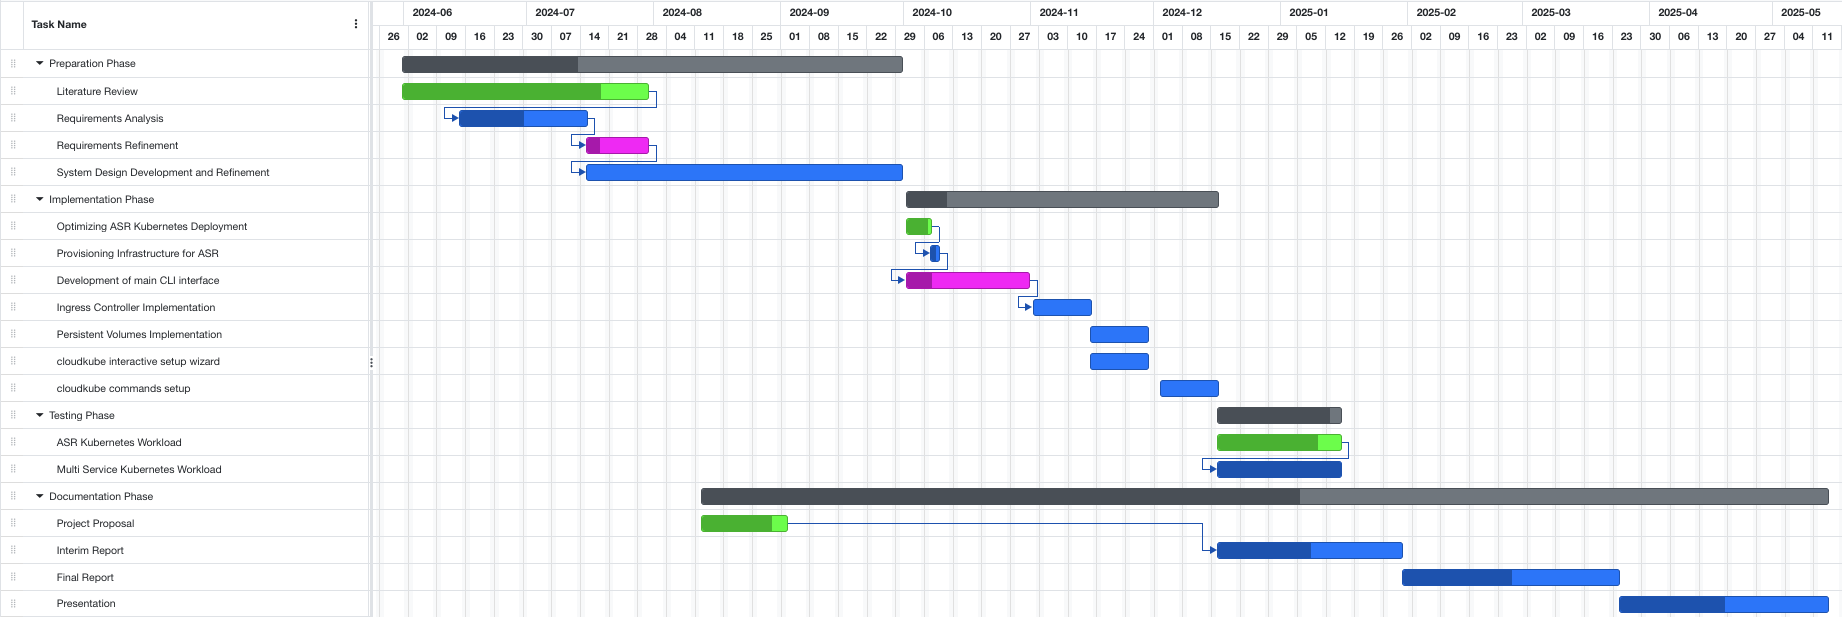
\includegraphics[width=\textwidth]{fig/gantt_chart.png}
%     \caption{Gantt Chart for Project Schedule}
%     \label{fig:gantt_chart}
% \end{figure}

\section{Report Organisation}
This report is structured into 5 different chapters, each detailing different aspects of the project.

\textbf{Chapter 1 - Introduction: } This chapter presents the background and introduction of the project. In this chapter, I elucidate some of the motivations for this project, and a brief overview on the intended outcome of this project.

\textbf{Chapter 2 - Literature Review: } This chapter reviews relevant technologies, and builds a foundational understanding for technical terminology used in future chapters. For completeness, this chapter will also discuss some of the pros and cons of each technology, which become relevant in later chapters.

\textbf{Chapter 3 - Planning and Design: } This chapter focuses on the analysis and design of the proposed solutions. In this chapter, I explore the current methods for handling containerised workloads, and show an optimized workflow for my proposed application.

\textbf{Chapter 4 - Implementation: } This chapter delves into the implementation of the proposed solutions. In this chapter, I detail the code and architecture used for \texttt{cloudkube}.

\textbf{Chapter 5 - Results and Analysis: } This chapter discusses the results of my proposed application, \texttt{cloudkube}. In this chapter, we will see the deployment of two applications to a Kubernetes environment provisioned by \texttt{cloudkube} - (1) ASR Application, and (2) Multi-service Kubernetes Application.

\textbf{Chapter 6 - Conclusion and Future Work: } This chapter presents the conclusions and recommendations for future work. 
\chapter{Literature Review}
To determine the most optimal design and implementation tool, I conducted a comprehensive evaluation of the various cloud technologies. This involved exploring the capabilities of each cloud technology, and diving into the supporting documentation. By understanding the objectives, strengths, and weaknesses of each of the different technologies, I was able to narrow down on the problem that I was trying to solve, and select the best tools that will align with the requirements of the project.

\section{Infrastructure as Code (IaC)}
According to AWS, “Infrastructure as Code (IaC) is the ability to provision and support your computing infrastructure using code instead of manual processes and settings.”. In the typical software development life cycle, when it gets to deploying applications, developers have to regularly set up, update, and maintain infrastructure in order to develop, test, and deploy applications \cite{aws-iac}. 

With more and more applications coming up, and companies focusing on high velocity, it has become increasingly important for these manual tasks like infrastructure provisioning to be automated. Furthermore, manual infrastructure provisioning is also more error prone, especially when managing applications at scale (AWS, n.d.). As such, more and more IaC tools have come up, so that infrastructure can be provisioned reliably, quickly, and unambiguously to support our applications in the cloud. Next, we will discuss some of the common IaC tools, their uses cases, strengths as well as pitfalls. 



\subsection{Terraform}
Perhaps one of the most popular IaC tools is Terraform. Terraform is an open-source IaC tool created by HashiCorp, which allows users to define and provision infrastructure declaratively. With Terraform, one can specify infrastructure resource in human-readable configuration files that can be reused, distributed, and modified \cite{cloud-2023}. 

\textbf{\textit{Benefits}}
\begin{enumerate}
\vspace{-1em}
    \item \textbf{Flexibility and Scalability:} Terraform integrates with over 1700 service providers governing different types of resources and services \cite{cloud-2023}, which means that developers can automate the deployment and management of a wide variety of resources ranging from compute instances to storage solutions.
    \item \textbf{Cloud Agnostic:} Terraform is cloud agnostic, meaning that a single configuration can manage multiple providers and handle cross-cloud dependencies.
    \item \textbf{Open Source:} Terraform is open source and free to use.
    \item \textbf{State Management:} Terraform manages its own state, meaning that cloud resources created and destroyed are all kept track of in a Terraform state file. This eliminates the worry of dangling or failed-to-provision resources.
\end{enumerate}

\textbf{\textit{How Terraform Works}}
\vspace{-1em}
\begin{enumerate}
    \item \textbf{Providers:} At a high level, Terraform creates resources based on the targets exposed application programming interfaces (APIs). Communication with these APIs happens through providers, which are plugins that interact with various platforms and manage their resources. These providers can be seen as a logical abstraction of an upstream API. Today, Terraform supports over 1800 providers, including major cloud providers such as AWS and GCP, as well as providers for Docker, Kubernetes, and more \cite{cvitkovic-2022}. Providers are normally defined in a top-level \texttt{terraform.tf} file as shown below:
    \begin{verbatim}
terraform {
  required_providers {
    aws = {
      source  = "hashicorp/aws"
      version = "~> 5.47.0"
    }
  }
  required_version = "~> 1.3"
}
    \end{verbatim}
    \item \textbf{terraform plan:} This command creates an execution plan, which generates a preview of the changes that Terraform plans to make to your infrastructure \cite{hashicorp}. By default, the following steps are taken:
    \begin{enumerate}
        \item Reads the current state of any already-existing remote objects to ensure that the Terraform state is up-to-date.
        \item Compares the current configuration to the prior state and generates a difference between the current and prior state.
        \item Proposes a set of changes that, if applied, will make the remote objects match the configuration.
    \end{enumerate}
    \item \textbf{terraform apply:} This command executes the actions proposed in a Terraform plan \cite{hashicorp}. By default, the following steps are taken:
    \begin{enumerate}
        \item All the steps as detailed in the above section on \texttt{terraform plan}.
        \item Prompt for plan approval. For auto-approval, the flag \texttt{--auto-approve} can also be passed to the \texttt{terraform apply} command.
        \item Undertakes the actions as indicated in the plan to modify existing cloud infrastructure to meet the desired current state.
        \item Modifies the state file to match the current state.
    \end{enumerate}
    \item \textbf{terraform destroy:} This command is used as a way to destroy all remote objects managed by a particular Terraform configuration \cite{hashicorp}.
    \item \textbf{The Terraform State File:} To make all of the above possible, Terraform needs to maintain some kind of state, so that it is aware of the current state of resources on the cloud. This is done through the \texttt{terraform.tfstate} file, which is automatically generated/modified on every Terraform command that mutates state. For local development of Terraform, the \texttt{terraform.tfstate} file is generated locally. For production and other higher environments, it is standard practice for the \texttt{terraform.tfstate} file to be stored in the cloud, such as an S3 bucket, with DynamoDB for locking, to ensure effective version control \cite{deepeshjaiswal-2024}.
\end{enumerate}

\begin{figure}[h!]
    \centering
    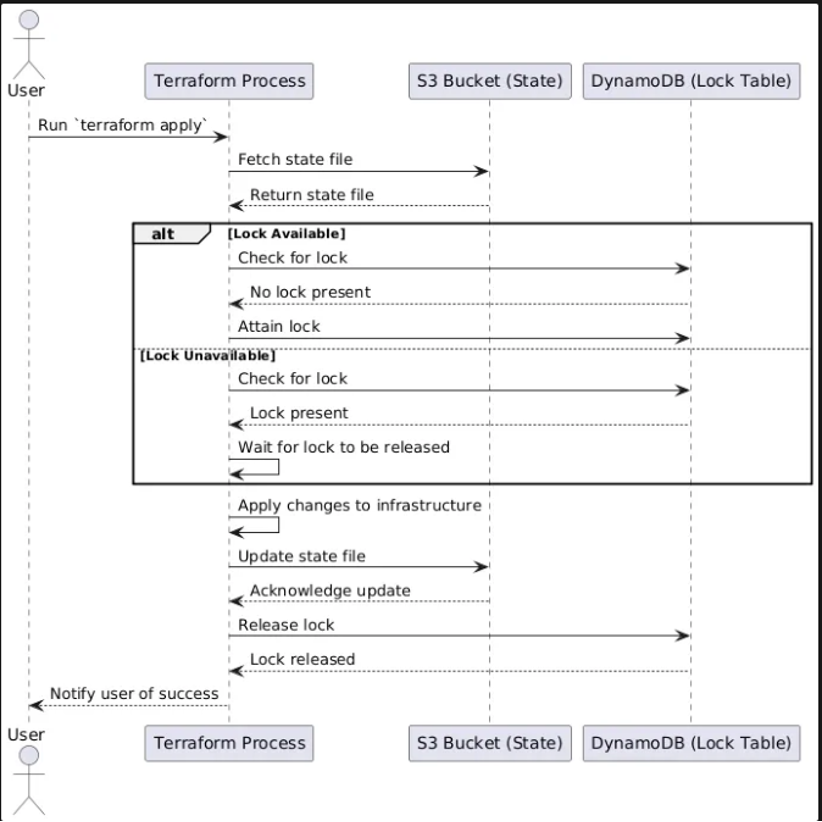
\includegraphics[width=0.8\textwidth]{fig/typical-tf-backend.png}
    \caption{Sequence Diagram for Terraform Backend}
    \label{fig:tf-backend}
\end{figure}

The above diagram shows the typical workflow in handling terraform state files. In summary, state files are usually saved to some storage such as an S3 bucket. Access to these state files are then synchronized via a lock, which is commonly implemented in DynamoDB \cite{deepeshjaiswal-2024}. This allows race-free interaction with the provisioned infrastructure.


\subsection{AWS CloudFormation}
AWS CloudFormation is an IaC tools that allows one to manage infrastructure and automate any deployments using code \cite{aws-cloudformation}. CloudFormation is also done declaratively, and written in familiar languages such as YAML or JSON. This makes managing, scaling, and automating AWS resources fast and straightforward. However, the greatest downside is that CloudFormation is part of the AWS stack, and is not cloud agnostic. This means that developers are reliant on the AWS cloud should they choose to use AWS CloudFormation. 

\subsection{OpenTofu}
OpenTofu is yet another open-source IaC tool designed to help with the provisioning and management of infrastructure \cite{dinu-2024}. It holds many similarities to Terraform as discussed above, but has an added feature of allowing for state encryption. There are also some differences in their licensing which will not be discussed here. 

\subsection{Ansible}
Ansible is an open-source automation tool used for configuration management, application deployment, and task automation. Unlike Terraform and CloudFormation, which are declarative, Ansible uses an imperative approach to define the desired state of the infrastructure. The greatest upside of Ansible is that it is agentless, meaning it does not require any software to be installed on the target machines.

\section{IaC Orchestration and Frameworks}
IaC orchestration is used to enforce good programming practices, improving code readability and quality. This provides additional structure, automation, and improves maintainability for complex infrastructure. These tools provide a significant advantage over pure Terraform by improving code readability, promoting consistency across projects, and enabling faster collaboration and development in multi-environment setups. 

Several IaC orchestration tools have also been built on top of terraform, such as terragrunt and terraspace. While an IaC orchestration tool will not be used in the implementation due to the main aim of keeping cloudkube portable and easily distributable, it is important to note how these tools fit into the whole cloud ecosystem.

\subsection{Terragrunt}
Terragrunt is a thin wrapper that is written on top of terraform, that provides some tooling and opinions \cite{nguyen-2020}. Terragrunt also provides a way to keep your code DRY by using the generate helper method. Terragrunt also helps in the automated creation of backends, which can be a chore if using raw terraform. Lastly, terragrunt allows for the injection of CLI hooks, allowing the utility to execute custom actions before or after terraform commands

\subsection{Terraspace}
Terraspace is a framework, which allows developer to dynamically generate terraform project in a centralized manner \cite{nguyen-no-date}. It is highly opinionated, and strongly enforces modularity and DRYness through stacks. On top of all the benefits offered by terragrunt, terraspace also allows the easy segregation of development and high-level environments through terraspace layering, which allows for the usage of the same code to deploy and create multiple environments. 

\section{Container and Container Orchestration}
Containerisation has become the standard practice of the industry today. Allowing for quicker software development cycles, together with more efficient CI/CD practices and portability, containerisation provides us a powerful, and agile way to manage our applications \cite{rgs-2023}. Along with the growing complexity of distributed systems, container orchestration software such as Kubernetes are also used to automate deployment, handle scalability and fault tolerance, as well as efficient resource utilization.
This chapter will discuss some of the common container and container orchestration software, which are pertinent to this project given that most SpeechLab applications have been containerised for the cloud

\subsection{Docker}
Docker is a containerisation software which aids in development, shipping, and deployment. Docker enables the separation of application from infrastructure so that software can be delivered quickly and reliably \cite{docker-docs-2024}. With docker, code, as well as version-locked dependencies are baked into a container image. This means that anyone building from this image on any machine in the world, regardless of architecture, will build the same thing, and run the same application. This creates reproducible environments of an application based on a single Docker Image. 

\subsection{Kubernetes}
Kubernetes is an open-source container orchestration software that helps to automate deployment, scale, and manage containerised applications. Kubernetes provides a framework to run distributed systems resiliently, taking care of scaling and failover of the application \cite{kubernetes-docs}. 

\textbf{\textit{Key Features of Kuberentes}}
\begin{enumerate}
    \vspace{-1em}
        \item \textbf{Self-healing: } Kubernetes restarts, replaces, or kills containers that are unhealthy, and doesn’t advertise these containers to clients until they are ready to serve.
        \item \textbf{Storage Orchestration:} Kubernetes allows the automatic mounting of a storage system of the developers choice.
        \item \textbf{Horizontal Scaling: } Kubernetes can scale up or down an application with a simple command, UI, or automatically based on user-defined parameters.
        \item \textbf{Service Discovery and Load Balancing: } Kubernetes can expose a container using the DNS name of the container, or using its own IP address. Kubernetes can also load balance and distribute network traffic to ensure deployment stability. 
\end{enumerate}

\textbf{\textit{Kubernetes Architecture}}
\begin{figure}[h!]
    \centering
    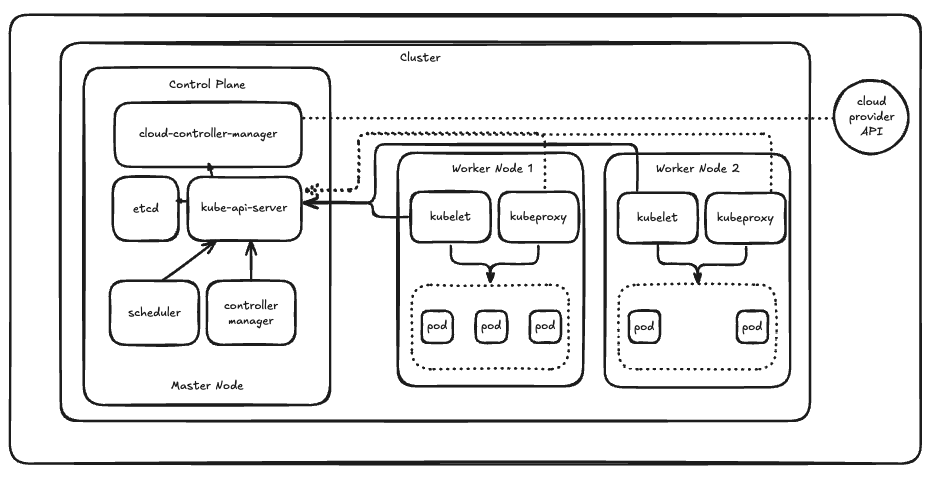
\includegraphics[width=1\textwidth]{fig/kubernetes-cluster-architecture.png}
    \caption{Typical Kubernetes Architecture}
    \label{fig:k8s-architecture}
\end{figure}

A Kubernetes cluster typically comprises the Control Plane as well as multiple Worker Nodes. Each of these nodes hold different responsibilities, which are detailed below.


\begin{enumerate}
    \vspace{-1em}
        \item \textbf{Master Node}
        \begin{enumerate}
            \item The Kubernetes master node, also known as the control plane, is the controller of the whole system. This is where all operational decisions are made, including scheduling, balancing, and responding to events.  
            \item \textit{kube-api-server:} The Kubernetes API Server is the main module within the master node which receives all REST requests for modifications, thereby serving as the frontend to the cluster \cite{bindlish-2021}. It acts as an interface for interaction with the cluster. 
            \item \textit{kube-controller-manager:} The kube-controller-manager runs a distict number of daemon processes, which help to regulate the shared state of the cluster, as well as perform routine tasks. When changes in configurations occur, the kcm is responsible for spotting the change and working toward the new desired state \cite{bindlish-2021}. 
            \item \textit{Kube-scheduler:}  The Kubernetes scheduler helps to schedule the pods on the various nodes based on resource utilization \cite{bindlish-2021}. The kube-scheduler is aware of all the resources available, and is responsible for allocating pods to nodes in an efficient manner to avoid resource exhaustion. Should no resources be available, the kube-scheduler puts pods in a pending state until resources are available again.
            \item \textit{etcd:} The etcd is a highly available, distributed key-value store that is use by Kubernetes to store cluster configuration data and state information. It keeps track of all cluster components such as nodes, pods, deployments and network configurations. 
        \end{enumerate}
        \item \textbf{Worker Nodes}
        \begin{enumerate}
            \item The Kubernetes worker node, is a worker machine in the Kubernetes cluster. There can be multiple worker nodes in a Kubernetes cluster. Each node is responsible for running pods, and is managed by the master node. These worker nodes are the workhorses of the Kubernetes cluster, and all application execution logic is carried out in these worker nodes. 
            \item \textit{kubelet:} The kubelet is the main service on a node, which regularly takes in pod specifications through the kube-api-server. The Kubelet is responsible for ensuring that pods and containers are healthy, and running in the desired state \cite{bindlish-2021}. The Kubelet is also responsible for health checks. 
            \item \textit{kube-proxy}: The kube-proxy is a service that runs on each worker node, that deals with networking. It is responsible for exposing services to the external world, or to the rest of the cluster. It performs request forwarding to the correct pods across various isolated networks in a cluster \cite{bindlish-2021}.
            \item \textit{Container runtime:} The container runtime is responsible for pulling images from a container image registry (i.e. Dockerhub, Amazon AWS ECR), and starting and stopping containers. The most common plugin used for this is Docker \cite{bindlish-2021}.
        \end{enumerate}
        \item \textbf{Pods}
        \begin{enumerate}
            \item A pod is the smallest unit that can be scheduled in Kubernetes \cite{bindlish-2021}. Pods help in scalability through replication. In the case of errors or failed health checks, Kubernetes also creates new pods, and destroys unhealthy ones. A single pod can contain multiple containers, and these containers share an IP address and port space, and are able to communicate internally via localhost.
        \end{enumerate}
\end{enumerate}

\textbf{\textit{Networking in Kubernetes}}

Another concept relevant to the development of \texttt{cloudkube} is networking in Kubernetes. The following section will two main networking concepts in Kubernetes, which will become relevant to our implementation in Chapter 4.
\begin{enumerate}
\item \textbf{Service: }A service in Kubernetes is a logical abstraction that provides stable networking for a group of pods running in a cluster. It enables communication between Pods, and ensures consistent access to applications, even if individual pods are created or deleted. These services can act as load balancers to distribute traffic across multiple pods. Pods with type \texttt{ClusterIP} work to expose services internally whthin the cluster. Pods with type \texttt{NodePort} exposes a service on a static port on each node, and pods with type \texttt{LoadBalancer} provisions an external load balancer in the cloud to publicly expose services. 
\item \textbf{Ingress: }A Kubernetes ingress object is an API object that manages external access to services in a cluster, typically through HTTP/HTTPS. The Ingress object allows us to map traffic to different backends based on rules defined via the Kubernetes API. 
\item \textbf{Ingress Controller: }In order for an Ingress to work in the cluster, there must be an ingress controller running. Ingress controllers are not started automatically with a cluster, and requires a one to be specified and provisioned for ingress resources to work. 
\end{enumerate}

\textbf{\textit{Storage in Kubernetes}}

Lastly, this section will detail how Kubernetes handles ephemeral and persistent storage. Similarly, this becomes relevant to our implementation as detailed in Chapter 4.
\begin{enumerate}
    \item \textbf{Volumes: } Volumes in Kubernetes provide a way for containers in a pod to access and share data via the filesystem. This can be used for data sharing between two different containers in the same pod, or even between two different pods. There are two broad categories of volumes. Ephemeral volume types have the lifetime of a pod, and follow the lifecycle of a pod, while persistent volumes exist beyond the lifetime of a pod.  
    \item \textbf{Persistent Volumes (PV): } A persistent volume is a piece of storage in the cluster that has been provisioned by the developer. The data in the PV remains even after pods are destroyed or recreated. 
    \item \textbf{Persistent Volume Claims (PVC): } A Persistent Volume Claim is a request for storage by a user. PVCs consume PV resources, and have defined access modes, such as ReadWriteOnce, ReadOnlyMany, ReadWriteMany, or ReadWriteOncePod. 
\end{enumerate}

\section{Infrastructure and Cloud}
This chapter details some of the key cloud infrastructure that is provisioned in order to host speech applications. For a proof of concept, and due to limited access to various clouds, everything in this paper is hosted on the AWS cloud. However, it should be noted that many of these concepts (such as VPC, subnets, load balancers etc.) are similar in other clouds, and \texttt{cloudkube} is extendable to other cloud providers as well. Each subsection will discuss the main uses of each of these components, and briefly detail the corresponding names of these components in AWS, Microsoft Azure Cloud, as well as Google Cloud Provider.

\begin{figure}[h!]
    \centering
    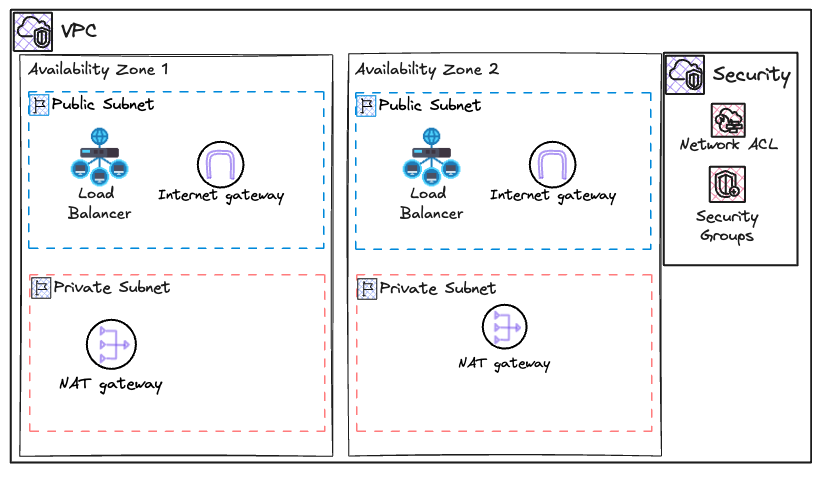
\includegraphics[width=\textwidth]{fig/vpc-subnets.png}
    \caption{Relationship between VPC, Subnets, and other basic cloud componenets}
    \label{fig:vpc-subnets}
\end{figure}


\subsection{Virtual Private Cloud (VPC)}
A virtual private cloud allows the creation of logically isolated sections of the cloud where different resources can be launched in a user-defined virtual network. Developers have full control over the virtual networking environment, including the selection of IP address ranges, creation of subnets, as well as configuration of route tables and network gateways. There will be mentions of some VPC related terminology in the following chapters, all of which are defined here.

\begin{itemize}
    \vspace{-1em}
    \item \textbf{Subnets: } Subnets allow the division of the VPC into different IP address ranges. They can be public or private.
    \item \textbf{Route Tables: } Route Tables allow the control of routing of traffic within the network. This helps in directing traffic between subnets, or between different VPCs.
    \item \textbf{Internet Gateway (IGW): } The Internet Gateway can be attached to a VPC to allow communication between resources in the VPC and the internet.
    \item \textbf{NAT Gateway: } The Network Address Translation (NAT) Gateway enables instances in a private subnet to connect to the internet or other cloud services while preventing the internet from initiating a connection with those instances.
    \item \textbf{Security Groups / Network Access Control Lists (ACLs): } These are virtual firewalls that control ingress and egress traffic at the instance and subnet levels, providing granular security controls.
\end{itemize}

\textbf{Cloud Provider VPCs}
\begin{itemize}
    \vspace{-1em}
\item AWS Cloud: AWS Virtual Private Cloud
\item GCP: Virtual Private Cloud Network
\item Microsoft Azure: Virtual Networks
\end{itemize}

\subsection{Subnets}
A subnet is a range of IP addresses in a VPC. Subnets allow us to segment the network inside the VPC to group resources and control their access to each other and to the outside world. A subnet can be thought of as a sub-network within a VPC, where resources like EC2 instances can reside.  

\textbf{Key Features of Subnets}
\begin{enumerate}
    \vspace{-1em}
\item Public and Private Subnets
    \begin{itemize}
    \item Public Subnets are subnets with a route to an IGW. Instances within this subnet can directly communicate with the internet, provided that they have a public IP address or an Elastic IP.
    \item Private subnets are subnets which do not have a route to an IGW. Instances in a private subnet cannot communicate with the internet directly. They can only access the internet via a NAT Gateway, or NAT instances in a public subnet.
    \end{itemize}
\item CIDR Blocks (Classless Interdomain Routing)
 \begin{itemize}
    \item Each subnet is associated with a CIDR block that defines its IP address range. CIDR blocks of subnets are always within (longer prefix mask) the CIDR block of the VPC.
\end{itemize}
\item Availability Zones (AZ)
\begin{itemize}
    \item Subnets are created within a specific AZ in a region. Resources within a subnet are guaranteed to be located within the same AZ.
    \item Distribution of subnets across multiple AZs help to increase availability and fault tolerance. 
\end{itemize}
\item NACLs
\begin{itemize}
    \item Subnets are protected using NACLs, which are stateless firewalls that operate at the subnet level. They control ingress and egress traffic to and from the subnets based on user-defined rules.  
    
\end{itemize}
\end{enumerate}

\subsection{Virtual Machines}
Kubernetes applications that run in the cloud require compute to be done on virtual machines. Virtual machines are web services offered by cloud providers which allow users to run virtual servers in the cloud. The virtual machines are normally configurable in terms of the choice of processor, storage, networking as well as operating systems. 

\textbf{Cloud Provider Virtual Machines}
\begin{itemize}
    \vspace{-1em}
\item AWS Cloud: AWS Elastic Compute Cloud (EC2)
\item GCP: Google Compute Engine (GCE)
\item Microsoft Azure: Azure Virtual Machine (VM)
\end{itemize}

Pertinent to this paper, EC2 instances will be provisioned as nodes in the Kubernetes cluster. The Kubernetes pods are then ultimately run on these nodes.  

\subsection{Security Groups}
Security groups are virtual firewalls that control inbound and outbound traffic to and from resources. Security groups are stateful, meaning that if you allow an incoming request from a particular IP address and port, the response is automatically allowed without needing a separate outbound rule. Some cloud providers such as Azure also draw a distinction between security groups which operate at the application layer (operating on compute instances and services), as well as the network layer (operating on ingress and egress IP addresses and protocols).

\subsection{Elastic Network Interfaces (ENI)}
An ENI is a logical networking component in a VPC that represents a virtual network card. These ENIs are attached to instances launched in the same AZ. Every VM instance has a primary ENI attached by default, providing the instance with networking capabilities. These ENIs have multiple use cases. Pertinent to this paper, the ENIs are used to facilitate communication between the Kubernetes control plane and worker nodes within the cluster.  

\subsection {Instance Templates}

Instance Templates allow users to define the configuration for launch VM instances in a more flexible and reusable way. They allow the specification of instance parameters such as instance type, key pair, security groups and more. These templates can then be used by Auto Scaling Groups, Spot Fleets, and other services to provision VM instances according to the configurations specified. 

\textbf{Cloud Provider Instance Templates}
\begin{itemize}
    \vspace{-1em}
\item AWS Cloud: AWS Launch Template
\item GCP: Instance Templates
\end{itemize}

Appendix \ref{appendix:cloudformation-eks-vpc-yaml} shows an example AWS Launch Template to provision a VPC for use with Kubernetes.

\subsection{Managed Kubernetes Service}

Managed Kubernetes Services are services offered by cloud providers which can be used to run Kubernetes without needing to install, operate, and maintain your own Kubernetes control plane or nodes. The managed Kubernetes service is able to automatically scale control plane instances based on load, detect and replace unhealthy control plane instances, and provide automated version updates and patching for them. These managed service also often offer easy integrability with other cloud services such as file systems for persistent volume storage, and load balancing for load distribution.

\textbf{Cloud Provider Managed Kubernetes Service}
\begin{itemize}
    \vspace{-1em}
\item AWS Cloud: Elastic Kubernetes Service (EKS)
\item GCP: Google Kubernetes Engine (GKE)
\item Microsoft Azure: Azure Kubernetes Service (AKS)
\end{itemize}

\subsection{File Systems}
File systems provide a simple, serverless, set-and-forget elastic file system for use with cloud resources or on premise infrastructure. They are built to scale on demand to petabytes without disrupting applications, growing and shrinking automatically as files are added or removed, thereby eliminating the need to provision and manage capacity to accommodate growth. 

\textbf{Cloud Provider File Systems}
\begin{itemize}
    \vspace{-1em}
\item AWS Cloud: Elastic File System (EFS)
\item GCP: Cloud Filestore
\item Microsoft Azure: Fileshare
\end{itemize}

\subsection{Scaling Groups}
Often times, it is important for compute instances to automatically scale with load. Scaling groups are a collection of compute instances treated as a logical grouping. Its main purpose and objective is to provide for automatic scaling and management. This allows the user to maintain the number of instances in a scaling group. The scaling group starts by launching enough instances to meet its desired capacity. It then maintains this number of instances by conducting periodic health checks on instances in the group. If an instance becomes unhealthy, the scaling group then terminates the instance and launches another instance to replace it.  

\textbf{Cloud Provider Scaling Groups}
\begin{itemize}
    \vspace{-1em}
\item AWS Cloud: Auto Scaling Groups (ASG)
\item GCP: Managed Instance Groups (MIG)
\item Microsoft Azure: Azure Virtual Machine Scale Sets (VMSS)
\end{itemize}

\subsection{minikube}
minikube is a way for one to quickly set up a local Kubernetes cluster. It is compatible with macOS, Linux and Windows. The main goal of minikube is to help application developers do quick testing of their Kubernetes deployments locally, as well as a tool used for learning by new Kubernetes users \cite{minikube-docs}. By default, minikube creates a one-node cluster locally, and supports addons such as ingress controllers. As we will see in the following chapter, cloudkube functionality closely mirrors that of minikube, supporting the objective of cloudkube which is to provide a quick and easy testing environment for Kubernetes developers in the cloud.

\section{Past FYPs}
Past FYPs have worked on the deployment of Speech Recognition Systems to on-prem bare metal resources \cite{yap-2023}, as well as the AWS Cloud.
Benjamin Chen and Poh Kai Kiat worked to set up the CI/CD pipelines for versioning of the ASR system using Jenkins, ArgoCD and Gitlab \cite{chen-2021} \cite{poh-2022}. 
Tjandy Putra's work helped to bolster security measures through Kyverno and Falco \cite{putra-2023}. Ma Xiao helped to set up the 
barebones deployment of the Speech Recognition System on the AWS cloud via the AWS console \cite{ma-2021}. Lastly, Song Yu and Lee Kai Shern
introduced terraform to help handle the infrastructure provisioning \cite{song-yu-2023} \cite{lee-2022}. 

These FYPs have done great work in deploying the ASR application. However, the deployment process is inherently tightly coupled with the 
ASR application, and changes to source code or structure of the application requires significant recalibration of cloud resources. As such, this 
FYP aims abstract away the process of infrastructure provisioning, and provide an automated tool for a Kubernetes cluster to be spun up easily in the cloud. 
As a stretch goal, this FYP also aims to be extendable to other SpeechLab applications. This will allow SpeechLab developers to focus on core application logic, and 
simply call the \texttt{cloudkube} API to spin up a Kuberenetes cluster, and deploy their applications. 
\chapter{Planning and Design}
\section{Traditional Approaches}
This section explores existing solutions like AWS ECS...

\chapter{Implementation}
Details on CloudKube’s architecture and workflow...

\chapter{Results and Analysis}
Analysis of deployment times, cost savings, and usability...

\chapter{Conclusion and Future Work}
CloudKube simplifies Kubernetes deployment...

%==== ENDING PART ===
  \clearpage
  \pagenumbering{arabic}%
  \renewcommand{\thepage}{R-\arabic{page}}
\lhead{}
\rhead{References}
\printbibliography[title={References}]

%=================================
\newpage
\appendix
\include{Appendices/appendix_a}
\chapter{Appendix B: VPC Requirements for EKS Cluster in AWS}
\label{appendix:eks-vpc-requirements}

The following are the VPC requirements for deploying an EKS Cluster in AWS.
\vspace{-1em}
\begin{enumerate}
    \item The VPC must have sufficient IP addresses for the cluster, any nodes, and Kubernetes resources that are created.
    \item If IPv6 is used by Kubernetes, then IPv6 CIDR blocks must be associated with the VPC and corresponding subnets.
    \item The VPC must have DNS hostname and DNS resolution support.
    \item The subnets must have at least six IP addresses for use by EKS.
    \item The subnets must be in at least two AZs.
    \item If inbound access is required from internet to pods, then there needs to be at least 1 public subnet with enough available IP addresses to deploy load balancers and ingresses to. 
    
\end{enumerate}




\chapter{Appendix C: AWS EKS Add-ons}
\label{appendix:aws-eks-addons}

\begin{figure}[h!]
    \centering
    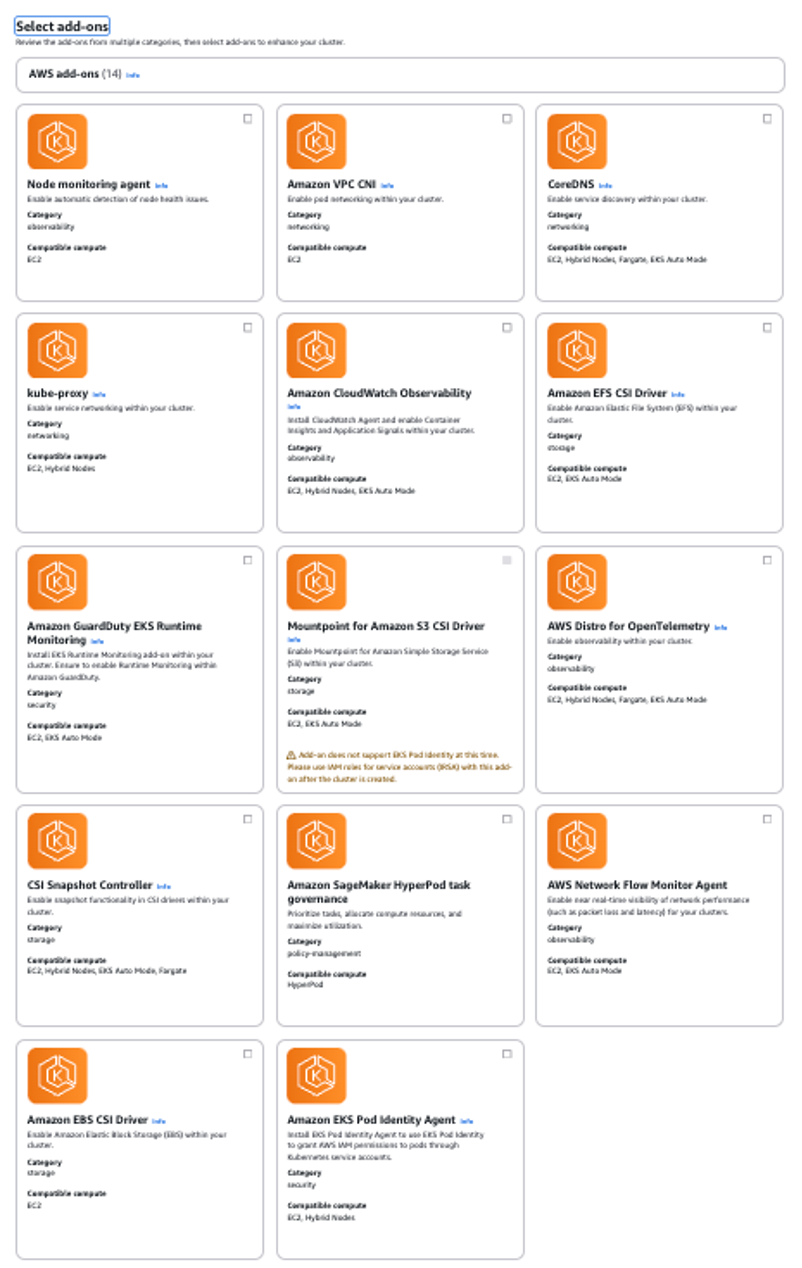
\includegraphics[width=0.75\textwidth]{fig/aws-eks-addons.png}
    \caption{AWS EKS Optional Add-ons}
    \label{fig:aws-eks-addons}
\end{figure}
\chapter{Appendix C: \texttt{cloudkube} README}
\label{appendix:cloudkube-readme}




\section*{\texttt{cloudkube} Developer Documentation}

\subsection*{Initial Setup}

The initial setup for \texttt{cloudkube} is straightforward and needs to be done only once. Since \texttt{cloudkube} runs on Python (\texttt{>= 3.11}), it is recommended to use virtual environments to avoid dependency conflicts and keep your global environment clean. Virtual environments can be created using \textbf{conda} (recommended), \textbf{pipenv}, or \textbf{python venv}.

\begin{enumerate}[leftmargin=4pt]
    \item \textbf{Create and Activate a Virtual Environment:}
          Use your preferred method (e.g., conda, pipenv, or venv) to create and activate a virtual environment.

    \item \textbf{Install \texttt{cloudkube}:}
          Run the following command to install \texttt{cloudkube} via \texttt{pip}:
          \begin{lstlisting}
pip install cloudkube
          \end{lstlisting}

    \item \textbf{Verify Installation:}
          Check if \texttt{cloudkube} was installed successfully:
          \begin{lstlisting}
pip list | grep cloudkube
          \end{lstlisting}

    \item \textbf{Install AWS CLI:}
          Follow the official AWS documentation to install the AWS CLI: 
          \href{https://docs.aws.amazon.com/cli/latest/userguide/getting-started-install.html}{\color{blue}\underline{Getting Started with AWS CLI}}.
          Configure your cloud credentials:
          \begin{lstlisting}
aws configure
          \end{lstlisting}
          For additional details, refer to the 
          \href{https://docs.aws.amazon.com/cli/latest/userguide/cli-chap-welcome.html}{\color{blue}\underline{AWS CLI Welcome Guide}}.

    \item \textbf{Install Terraform:}
          \begin{itemize}[leftmargin=4pt]
              \item \textbf{macOS (Recommended):}
                    Install Terraform using Homebrew:
                    \begin{lstlisting}
brew tap hashicorp/tap
brew install hashicorp/tap/terraform
brew update
brew upgrade hashicorp/tap/terraform
                    \end{lstlisting}

              \item \textbf{Other Platforms:}
                    Terraform can also be installed on other platformrs by following the \href{https://developer.hashicorp.com/terraform/tutorials/aws-get-started/install-cli}{\color{blue}\underline{Terraform Developer Documentation}}.
          \end{itemize}

    \item \textbf{Verify Terraform Installation:}
          \begin{lstlisting}
terraform -version
          \end{lstlisting}
\end{enumerate}

Once all dependencies are installed, you are ready to start using \texttt{cloudkube}!

\subsection*{\texttt{cloudkube} Workflow}

\subsubsection*{1. Initialize \texttt{cloudkube}}
To start working with cloudkube, run `cloudkube init`. This will bring up and interactive wizard, which will bring you through the provisioning of a cluster. 
\begin{lstlisting}
cloudkube init
\end{lstlisting}
This starts an interactive wizard to guide you through the provisioning of a Kubernetes cluster.

\subsubsection*{2. Configure Cluster Configuration}
\begin{enumerate}
    \item In the wizard, select \textbf{Option 2} to configure the cluster.
    \item Provide the following information when prompted:
          \begin{itemize}
              \item Name of the cluster
              \item Region
              \item Compute architecture
              \item Optional add-ons (e.g., persistent volumes, ingress controllers)
          \end{itemize}
    \item The configuration details will be saved in a file named \texttt{config.json} in the same directory where \texttt{cloudkube} is run.
\end{enumerate}

\subsubsection*{3. Spin Up the Cluster}
\begin{enumerate}
    \item Select \textbf{Option 3} in the interactive wizard.
    \item \texttt{cloudkube} performs the following actions:
          \begin{itemize}
              \item \texttt{terraform init}: Installs all required Terraform dependencies and sets up the environment.
              \item \texttt{terraform plan}: Creates a resource plan and seeks user approval before proceeding.
              \item \texttt{terraform apply}: Provisions the required infrastructure, including:
                    \begin{itemize}
                        \item An EKS-compliant VPC
                        \item Relevant permissions and security groups
                    \end{itemize}
              \item Automatically configures the local environment to communicate with the cluster by populating \texttt{\textasciitilde/.kube/config}.
          \end{itemize}
\end{enumerate}

\subsubsection*{4. Verify Cluster Creation}
\begin{enumerate}
    \item Check the cluster creation via the \textbf{AWS Console}.
    \item Use the following \texttt{kubectl} commands for further verification:
          \begin{itemize}
              \item List all pods:
                    \begin{lstlisting}
kubectl get pods -A
                    \end{lstlisting}
              \item List all nodes:
                    \begin{lstlisting}
kubectl get nodes
                    \end{lstlisting}
          \end{itemize}
\end{enumerate}

\subsubsection*{5. Apply Kubernetes Manifests}
To deploy your application:
\begin{enumerate}
    \item Ensure your Kubernetes YAML files are stored in the \texttt{./kubernetes} directory.
    \item Apply the manifests:
          \begin{lstlisting}
kubectl apply -f ./kubernetes
          \end{lstlisting}
\end{enumerate}

\subsubsection*{6. Teardown and Resource Deprovisioning}
Once you are done testing your application:
\vspace{-1em}
\begin{enumerate}
    \item Remove your Kubernetes deployment:
          \begin{lstlisting}
kubectl delete -f ./kubernetes
          \end{lstlisting}
    \item Run the following command and select \textbf{Option 4} in the wizard to:
          \begin{itemize}
              \item Deprovision all resources
              \item Clean up your local Kubernetes configuration file (\texttt{\textasciitilde/.kube/config}):
                    \begin{lstlisting}
cloudkube init
                    \end{lstlisting}
          \end{itemize}
\end{enumerate}

\subsection*{Notes}
\begin{itemize}
    \item As of version \texttt{v1.0}, \texttt{cloudkube} only supports \textbf{AWS Cloud}. If support for other cloud providers is added in the future, their respective setup steps should be followed.
    \item Ensure that the EKS cluster meets all networking and security requirements specified in the AWS documentation.
\end{itemize}


\chapter{Appendix D: terraform plan output for \texttt{cloudkube} provisioning}
\label{appendix:cloudkube-provision-tf-plan}

The following refers to a part of the output after selection Option 3 in the \texttt{cloudkube} CLI. This is the output redirected 
from \texttt{stdout} of \texttt{terraform plan}. 

\begin{lstlisting}[caption={terraform plan output for \texttt{cloudkube} provisioning}, breaklines=true, breakatwhitespace=false]
    module.eks.module.eks_managed_node_group["one"].data.aws_partition.current: Reading...
    module.eks.data.aws_iam_policy_document.assume_role_policy[0]: Reading...
    module.eks.data.aws_caller_identity.current: Reading...
    module.eks.data.aws_partition.current: Reading...
    module.eks.module.eks_managed_node_group["one"].data.aws_caller_identity.current: Reading...
    module.eks.module.kms.data.aws_partition.current[0]: Reading...
    module.eks.module.eks_managed_node_group["one"].data.aws_iam_policy_document.assume_role_policy[0]: Reading...
    module.eks.module.kms.data.aws_caller_identity.current[0]: Reading...
    module.eks.module.kms.data.aws_partition.current[0]: Read complete after 0s [id=aws]
    module.eks.module.eks_managed_node_group["one"].data.aws_partition.current: Read complete after 0s [id=aws]
    module.eks.module.eks_managed_node_group["one"].data.aws_iam_policy_document.assume_role_policy[0]: Read complete after 0s [id=2560088296]
    module.eks.data.aws_partition.current: Read complete after 0s [id=aws]
    module.eks.data.aws_iam_policy_document.assume_role_policy[0]: Read complete after 0s [id=2764486067]
    module.eks.data.aws_caller_identity.current: Read complete after 0s [id=861814105207]
    module.eks.data.aws_iam_session_context.current: Reading...
    module.eks.data.aws_iam_session_context.current: Read complete after 0s [id=arn:aws:iam::861814105207:user/chanming]
    module.eks.module.kms.data.aws_caller_identity.current[0]: Read complete after 0s [id=861814105207]
    module.eks.module.eks_managed_node_group["one"].data.aws_caller_identity.current: Read complete after 0s [id=861814105207]
    
    Terraform used the selected providers to generate the following execution plan. Resource actions are indicated with the following symbols:
      + create
     <= read (data resources)
    
    Terraform will perform the following actions:
    
      # aws_efs_backup_policy.policy will be created
      + resource "aws_efs_backup_policy" "policy" {
          + file_system_id = (known after apply)
          + id             = (known after apply)
    
          + backup_policy {
              + status = "ENABLED"
            }
        }
    
      # aws_efs_file_system.efs will be created
      + resource "aws_efs_file_system" "efs" {
          + arn                     = (known after apply)
          + availability_zone_id    = (known after apply)
          + availability_zone_name  = (known after apply)
          + creation_token          = "minghan-eks-cluster-efs-filesystem"
          + dns_name                = (known after apply)
          + encrypted               = true
          + id                      = (known after apply)
          + kms_key_id              = (known after apply)
          + name                    = (known after apply)
          + number_of_mount_targets = (known after apply)
          + owner_id                = (known after apply)
          + performance_mode        = (known after apply)
          + size_in_bytes           = (known after apply)
          + tags_all                = (known after apply)
          + throughput_mode         = "elastic"
    
          + lifecycle_policy {
              + transition_to_ia = "AFTER_30_DAYS"
            }
    
          + protection (known after apply)
        }
    
      # aws_efs_mount_target.efs_mount_target_1 will be created
      + resource "aws_efs_mount_target" "efs_mount_target_1" {
          + availability_zone_id   = (known after apply)
          + availability_zone_name = (known after apply)
          + dns_name               = (known after apply)
          + file_system_arn        = (known after apply)
          + file_system_id         = (known after apply)
          + id                     = (known after apply)
          + ip_address             = (known after apply)
          + mount_target_dns_name  = (known after apply)
          + network_interface_id   = (known after apply)
          + owner_id               = (known after apply)
          + security_groups        = (known after apply)
          + subnet_id              = (known after apply)
        }
    
      # aws_efs_mount_target.efs_mount_target_2 will be created
      + resource "aws_efs_mount_target" "efs_mount_target_2" {
          + availability_zone_id   = (known after apply)
          + availability_zone_name = (known after apply)
          + dns_name               = (known after apply)
          + file_system_arn        = (known after apply)
          + file_system_id         = (known after apply)
          + id                     = (known after apply)
          + ip_address             = (known after apply)
          + mount_target_dns_name  = (known after apply)
          + network_interface_id   = (known after apply)
          + owner_id               = (known after apply)
          + security_groups        = (known after apply)
          + subnet_id              = (known after apply)
        }
    
      # aws_security_group.efs_security_group will be created
      + resource "aws_security_group" "efs_security_group" {
          + arn                    = (known after apply)
          + description            = "Security group for EFS with NFS access"
          + egress                 = [
              + {
                  + cidr_blocks      = [
                      + "0.0.0.0/0",
                    ]
                  + from_port        = 0
                  + ipv6_cidr_blocks = []
                  + prefix_list_ids  = []
                  + protocol         = "-1"
                  + security_groups  = []
                  + self             = false
                  + to_port          = 0
                    # (1 unchanged attribute hidden)
                },
            ]
          + id                     = (known after apply)
          + ingress                = [
              + {
                  + cidr_blocks      = [
                      + "10.0.0.0/16",
                    ]
                  + description      = "Allow NFS access"
                  + from_port        = 2049
                  + ipv6_cidr_blocks = []
                  + prefix_list_ids  = []
                  + protocol         = "tcp"
                  + security_groups  = []
                  + self             = false
                  + to_port          = 2049
                },
            ]
          + name                   = "minghan-eks-cluster-efs"
          + name_prefix            = (known after apply)
          + owner_id               = (known after apply)
          + revoke_rules_on_delete = false
          + tags                   = {
              + "Name" = "minghan-eks-cluster-efs-nfs-sg"
            }
          + tags_all               = {
              + "Name" = "minghan-eks-cluster-efs-nfs-sg"
            }
          + vpc_id                 = (known after apply)
        }
    
      # random_string.suffix will be created
      + resource "random_string" "suffix" {
          + id          = (known after apply)
          + length      = 8
          + lower       = true
          + min_lower   = 0
          + min_numeric = 0
          + min_special = 0
          + min_upper   = 0
          + number      = true
          + numeric     = true
          + result      = (known after apply)
          + special     = false
          + upper       = true
        }
    
      # module.eks.data.aws_eks_addon_version.this["coredns"] will be read during apply
      # (depends on a resource or a module with changes pending)
     <= data "aws_eks_addon_version" "this" {
          + addon_name         = "coredns"
          + id                 = (known after apply)
          + kubernetes_version = "1.30"
          + version            = (known after apply)
        }
    
      # module.eks.data.aws_eks_addon_version.this["eks-pod-identity-agent"] will be read during apply
      # (depends on a resource or a module with changes pending)
     <= data "aws_eks_addon_version" "this" {
          + addon_name         = "eks-pod-identity-agent"
          + id                 = (known after apply)
          + kubernetes_version = "1.30"
          + version            = (known after apply)
        }
    
      # module.eks.data.aws_eks_addon_version.this["kube-proxy"] will be read during apply
      # (depends on a resource or a module with changes pending)
     <= data "aws_eks_addon_version" "this" {
          + addon_name         = "kube-proxy"
          + id                 = (known after apply)
          + kubernetes_version = "1.30"
          + version            = (known after apply)
        }
    
      # module.eks.data.aws_eks_addon_version.this["vpc-cni"] will be read during apply
      # (depends on a resource or a module with changes pending)
     <= data "aws_eks_addon_version" "this" {
          + addon_name         = "vpc-cni"
          + id                 = (known after apply)
          + kubernetes_version = "1.30"
          + version            = (known after apply)
        }
    
      # module.eks.data.tls_certificate.this[0] will be read during apply
      # (config refers to values not yet known)
     <= data "tls_certificate" "this" {
          + certificates = (known after apply)
          + id           = (known after apply)
          + url          = (known after apply)
        }
    
      # module.eks.aws_cloudwatch_log_group.this[0] will be created
      + resource "aws_cloudwatch_log_group" "this" {
          + arn               = (known after apply)
          + id                = (known after apply)
          + log_group_class   = (known after apply)
          + name              = (known after apply)
          + name_prefix       = (known after apply)
          + retention_in_days = 90
          + skip_destroy      = false
          + tags              = (known after apply)
          + tags_all          = (known after apply)
        }
    
      # module.eks.aws_eks_access_entry.this["cluster_creator"] will be created
      + resource "aws_eks_access_entry" "this" {
          + access_entry_arn  = (known after apply)
          + cluster_name      = (known after apply)
          + created_at        = (known after apply)
          + id                = (known after apply)
          + kubernetes_groups = (known after apply)
          + modified_at       = (known after apply)
          + principal_arn     = "arn:aws:iam::861814105207:user/chanming"
          + tags_all          = (known after apply)
          + type              = "STANDARD"
          + user_name         = (known after apply)
        }
    
      # module.eks.aws_eks_access_policy_association.this["cluster_creator_admin"] will be created
      + resource "aws_eks_access_policy_association" "this" {
          + associated_at = (known after apply)
          + cluster_name  = (known after apply)
          + id            = (known after apply)
          + modified_at   = (known after apply)
          + policy_arn    = "arn:aws:eks::aws:cluster-access-policy/AmazonEKSClusterAdminPolicy"
          + principal_arn = "arn:aws:iam::861814105207:user/chanming"
    
          + access_scope {
              + type = "cluster"
            }
        }
    
      # module.eks.aws_eks_addon.this["coredns"] will be created
      + resource "aws_eks_addon" "this" {
          + addon_name                  = "coredns"
          + addon_version               = (known after apply)
          + arn                         = (known after apply)
          + cluster_name                = (known after apply)
          + configuration_values        = (known after apply)
          + created_at                  = (known after apply)
          + id                          = (known after apply)
          + modified_at                 = (known after apply)
          + preserve                    = true
          + resolve_conflicts_on_create = "OVERWRITE"
          + resolve_conflicts_on_update = "OVERWRITE"
          + tags_all                    = (known after apply)
    
          + timeouts {}
        }
    
      # module.eks.aws_eks_addon.this["eks-pod-identity-agent"] will be created
      + resource "aws_eks_addon" "this" {
          + addon_name                  = "eks-pod-identity-agent"
          + addon_version               = (known after apply)
          + arn                         = (known after apply)
          + cluster_name                = (known after apply)
          + configuration_values        = (known after apply)
          + created_at                  = (known after apply)
          + id                          = (known after apply)
          + modified_at                 = (known after apply)
          + preserve                    = true
          + resolve_conflicts_on_create = "OVERWRITE"
          + resolve_conflicts_on_update = "OVERWRITE"
          + tags_all                    = (known after apply)
    
          + timeouts {}
        }
    
      # module.eks.aws_eks_addon.this["kube-proxy"] will be created
      + resource "aws_eks_addon" "this" {
          + addon_name                  = "kube-proxy"
          + addon_version               = (known after apply)
          + arn                         = (known after apply)
          + cluster_name                = (known after apply)
          + configuration_values        = (known after apply)
          + created_at                  = (known after apply)
          + id                          = (known after apply)
          + modified_at                 = (known after apply)
          + preserve                    = true
          + resolve_conflicts_on_create = "OVERWRITE"
          + resolve_conflicts_on_update = "OVERWRITE"
          + tags_all                    = (known after apply)
    
          + timeouts {}
        }
    
      # module.eks.aws_eks_addon.this["vpc-cni"] will be created
      + resource "aws_eks_addon" "this" {
          + addon_name                  = "vpc-cni"
          + addon_version               = (known after apply)
          + arn                         = (known after apply)
          + cluster_name                = (known after apply)
          + configuration_values        = (known after apply)
          + created_at                  = (known after apply)
          + id                          = (known after apply)
          + modified_at                 = (known after apply)
          + preserve                    = true
          + resolve_conflicts_on_create = "OVERWRITE"
          + resolve_conflicts_on_update = "OVERWRITE"
          + tags_all                    = (known after apply)
    
          + timeouts {}
        }
    
      # module.eks.aws_eks_cluster.this[0] will be created
      + resource "aws_eks_cluster" "this" {
          + arn                       = (known after apply)
          + certificate_authority     = (known after apply)
          + cluster_id                = (known after apply)
          + created_at                = (known after apply)
          + enabled_cluster_log_types = [
              + "api",
              + "audit",
              + "authenticator",
              + "controllerManager",
              + "scheduler",
            ]
          + endpoint                  = (known after apply)
          + id                        = (known after apply)
          + identity                  = (known after apply)
          + name                      = (known after apply)
          + platform_version          = (known after apply)
          + role_arn                  = (known after apply)
          + status                    = (known after apply)
          + tags                      = {
              + "terraform-aws-modules" = "eks"
            }
          + tags_all                  = {
              + "terraform-aws-modules" = "eks"
            }
          + version                   = "1.30"
    
          + access_config {
              + authentication_mode                         = "API_AND_CONFIG_MAP"
              + bootstrap_cluster_creator_admin_permissions = false
            }
    
          + encryption_config {
              + resources = [
                  + "secrets",
                ]
    
              + provider {
                  + key_arn = (known after apply)
                }
            }
    
          + kubernetes_network_config {
              + ip_family         = "ipv4"
              + service_ipv4_cidr = (known after apply)
              + service_ipv6_cidr = (known after apply)
            }
    
          + timeouts {}
    
          + vpc_config {
              + cluster_security_group_id = (known after apply)
              + endpoint_private_access   = true
              + endpoint_public_access    = true
              + public_access_cidrs       = [
                  + "0.0.0.0/0",
                ]
              + security_group_ids        = (known after apply)
              + subnet_ids                = (known after apply)
              + vpc_id                    = (known after apply)
            }
        }
    
      # module.eks.aws_iam_openid_connect_provider.oidc_provider[0] will be created
      + resource "aws_iam_openid_connect_provider" "oidc_provider" {
          + arn             = (known after apply)
          + client_id_list  = [
              + "sts.amazonaws.com",
            ]
          + id              = (known after apply)
          + tags            = (known after apply)
          + tags_all        = (known after apply)
          + thumbprint_list = (known after apply)
          + url             = (known after apply)
        }
    
      # module.eks.aws_iam_policy.cluster_encryption[0] will be created
      + resource "aws_iam_policy" "cluster_encryption" {
          + arn              = (known after apply)
          + attachment_count = (known after apply)
          + description      = "Cluster encryption policy to allow cluster role to utilize CMK provided"
          + id               = (known after apply)
          + name             = (known after apply)
          + name_prefix      = (known after apply)
          + path             = "/"
          + policy           = (known after apply)
          + policy_id        = (known after apply)
          + tags_all         = (known after apply)
        }
    
      # module.eks.aws_iam_role.this[0] will be created
      + resource "aws_iam_role" "this" {
          + arn                   = (known after apply)
          + assume_role_policy    = jsonencode(
                {
                  + Statement = [
                      + {
                          + Action    = "sts:AssumeRole"
                          + Effect    = "Allow"
                          + Principal = {
                              + Service = "eks.amazonaws.com"
                            }
                          + Sid       = "EKSClusterAssumeRole"
                        },
                    ]
                  + Version   = "2012-10-17"
                }
            )
          + create_date           = (known after apply)
          + force_detach_policies = true
          + id                    = (known after apply)
          + managed_policy_arns   = (known after apply)
          + max_session_duration  = 3600
          + name                  = (known after apply)
          + name_prefix           = (known after apply)
          + path                  = "/"
          + tags_all              = (known after apply)
          + unique_id             = (known after apply)
    
          + inline_policy {
              + name   = (known after apply)
              + policy = jsonencode(
                    {
                      + Statement = [
                          + {
                              + Action   = [
                                  + "logs:CreateLogGroup",
                                ]
                              + Effect   = "Deny"
                              + Resource = "*"
                            },
                        ]
                      + Version   = "2012-10-17"
                    }
                )
            }
        }
    
      # module.eks.aws_iam_role_policy_attachment.cluster_encryption[0] will be created
      + resource "aws_iam_role_policy_attachment" "cluster_encryption" {
          + id         = (known after apply)
          + policy_arn = (known after apply)
          + role       = (known after apply)
        }
    
      # module.eks.aws_iam_role_policy_attachment.this["AmazonEKSClusterPolicy"] will be created
      + resource "aws_iam_role_policy_attachment" "this" {
          + id         = (known after apply)
          + policy_arn = "arn:aws:iam::aws:policy/AmazonEKSClusterPolicy"
          + role       = (known after apply)
        }
    
      # module.eks.aws_iam_role_policy_attachment.this["AmazonEKSVPCResourceController"] will be created
      + resource "aws_iam_role_policy_attachment" "this" {
          + id         = (known after apply)
          + policy_arn = "arn:aws:iam::aws:policy/AmazonEKSVPCResourceController"
          + role       = (known after apply)
        }
    
      # module.eks.aws_security_group.cluster[0] will be created
      + resource "aws_security_group" "cluster" {
          + arn                    = (known after apply)
          + description            = "EKS cluster security group"
          + egress                 = (known after apply)
          + id                     = (known after apply)
          + ingress                = (known after apply)
          + name                   = (known after apply)
          + name_prefix            = (known after apply)
          + owner_id               = (known after apply)
          + revoke_rules_on_delete = false
          + tags                   = (known after apply)
          + tags_all               = (known after apply)
          + vpc_id                 = (known after apply)
        }
    
      # module.eks.aws_security_group.node[0] will be created
      + resource "aws_security_group" "node" {
          + arn                    = (known after apply)
          + description            = "EKS node shared security group"
          + egress                 = (known after apply)
          + id                     = (known after apply)
          + ingress                = (known after apply)
          + name                   = (known after apply)
          + name_prefix            = (known after apply)
          + owner_id               = (known after apply)
          + revoke_rules_on_delete = false
          + tags                   = (known after apply)
          + tags_all               = (known after apply)
          + vpc_id                 = (known after apply)
        }
    
      # module.eks.aws_security_group_rule.cluster["ingress_nodes_443"] will be created
      + resource "aws_security_group_rule" "cluster" {
          + description              = "Node groups to cluster API"
          + from_port                = 443
          + id                       = (known after apply)
          + protocol                 = "tcp"
          + security_group_id        = (known after apply)
          + security_group_rule_id   = (known after apply)
          + self                     = false
          + source_security_group_id = (known after apply)
          + to_port                  = 443
          + type                     = "ingress"
        }
    
      # module.eks.aws_security_group_rule.node["egress_all"] will be created
      + resource "aws_security_group_rule" "node" {
          + cidr_blocks              = [
              + "0.0.0.0/0",
            ]
          + description              = "Allow all egress"
          + from_port                = 0
          + id                       = (known after apply)
          + prefix_list_ids          = []
          + protocol                 = "-1"
          + security_group_id        = (known after apply)
          + security_group_rule_id   = (known after apply)
          + self                     = false
          + source_security_group_id = (known after apply)
          + to_port                  = 0
          + type                     = "egress"
        }
    
      # module.eks.aws_security_group_rule.node["ingress_cluster_443"] will be created
      + resource "aws_security_group_rule" "node" {
          + description              = "Cluster API to node groups"
          + from_port                = 443
          + id                       = (known after apply)
          + prefix_list_ids          = []
          + protocol                 = "tcp"
          + security_group_id        = (known after apply)
          + security_group_rule_id   = (known after apply)
          + self                     = false
          + source_security_group_id = (known after apply)
          + to_port                  = 443
          + type                     = "ingress"
        }
    
      # module.eks.aws_security_group_rule.node["ingress_cluster_4443_webhook"] will be created
      + resource "aws_security_group_rule" "node" {
          + description              = "Cluster API to node 4443/tcp webhook"
          + from_port                = 4443
          + id                       = (known after apply)
          + prefix_list_ids          = []
          + protocol                 = "tcp"
          + security_group_id        = (known after apply)
          + security_group_rule_id   = (known after apply)
          + self                     = false
          + source_security_group_id = (known after apply)
          + to_port                  = 4443
          + type                     = "ingress"
        }
    
      # module.eks.aws_security_group_rule.node["ingress_cluster_6443_webhook"] will be created
      + resource "aws_security_group_rule" "node" {
          + description              = "Cluster API to node 6443/tcp webhook"
          + from_port                = 6443
          + id                       = (known after apply)
          + prefix_list_ids          = []
          + protocol                 = "tcp"
          + security_group_id        = (known after apply)
          + security_group_rule_id   = (known after apply)
          + self                     = false
          + source_security_group_id = (known after apply)
          + to_port                  = 6443
          + type                     = "ingress"
        }
    
      # module.eks.aws_security_group_rule.node["ingress_cluster_8443_webhook"] will be created
      + resource "aws_security_group_rule" "node" {
          + description              = "Cluster API to node 8443/tcp webhook"
          + from_port                = 8443
          + id                       = (known after apply)
          + prefix_list_ids          = []
          + protocol                 = "tcp"
          + security_group_id        = (known after apply)
          + security_group_rule_id   = (known after apply)
          + self                     = false
          + source_security_group_id = (known after apply)
          + to_port                  = 8443
          + type                     = "ingress"
        }
    
      # module.eks.aws_security_group_rule.node["ingress_cluster_9443_webhook"] will be created
      + resource "aws_security_group_rule" "node" {
          + description              = "Cluster API to node 9443/tcp webhook"
          + from_port                = 9443
          + id                       = (known after apply)
          + prefix_list_ids          = []
          + protocol                 = "tcp"
          + security_group_id        = (known after apply)
          + security_group_rule_id   = (known after apply)
          + self                     = false
          + source_security_group_id = (known after apply)
          + to_port                  = 9443
          + type                     = "ingress"
        }
    
      # module.eks.aws_security_group_rule.node["ingress_cluster_kubelet"] will be created
      + resource "aws_security_group_rule" "node" {
          + description              = "Cluster API to node kubelets"
          + from_port                = 10250
          + id                       = (known after apply)
          + prefix_list_ids          = []
          + protocol                 = "tcp"
          + security_group_id        = (known after apply)
          + security_group_rule_id   = (known after apply)
          + self                     = false
          + source_security_group_id = (known after apply)
          + to_port                  = 10250
          + type                     = "ingress"
        }
    
      # module.eks.aws_security_group_rule.node["ingress_nodes_ephemeral"] will be created
      + resource "aws_security_group_rule" "node" {
          + description              = "Node to node ingress on ephemeral ports"
          + from_port                = 1025
          + id                       = (known after apply)
          + prefix_list_ids          = []
          + protocol                 = "tcp"
          + security_group_id        = (known after apply)
          + security_group_rule_id   = (known after apply)
          + self                     = true
          + source_security_group_id = (known after apply)
          + to_port                  = 65535
          + type                     = "ingress"
        }
    
      # module.eks.aws_security_group_rule.node["ingress_self_all"] will be created
      + resource "aws_security_group_rule" "node" {
          + description              = "Node to node all ports/protocols"
          + from_port                = 0
          + id                       = (known after apply)
          + prefix_list_ids          = []
          + protocol                 = "-1"
          + security_group_id        = (known after apply)
          + security_group_rule_id   = (known after apply)
          + self                     = true
          + source_security_group_id = (known after apply)
          + to_port                  = 0
          + type                     = "ingress"
        }
    
      # module.eks.aws_security_group_rule.node["ingress_self_coredns_tcp"] will be created
      + resource "aws_security_group_rule" "node" {
          + description              = "Node to node CoreDNS"
          + from_port                = 53
          + id                       = (known after apply)
          + prefix_list_ids          = []
          + protocol                 = "tcp"
          + security_group_id        = (known after apply)
          + security_group_rule_id   = (known after apply)
          + self                     = true
          + source_security_group_id = (known after apply)
          + to_port                  = 53
          + type                     = "ingress"
        }
    
      # module.eks.aws_security_group_rule.node["ingress_self_coredns_udp"] will be created
      + resource "aws_security_group_rule" "node" {
          + description              = "Node to node CoreDNS UDP"
          + from_port                = 53
          + id                       = (known after apply)
          + prefix_list_ids          = []
          + protocol                 = "udp"
          + security_group_id        = (known after apply)
          + security_group_rule_id   = (known after apply)
          + self                     = true
          + source_security_group_id = (known after apply)
          + to_port                  = 53
          + type                     = "ingress"
        }
    
      # module.eks.time_sleep.this[0] will be created
      + resource "time_sleep" "this" {
          + create_duration = "30s"
          + id              = (known after apply)
          + triggers        = {
              + "cluster_certificate_authority_data" = (known after apply)
              + "cluster_endpoint"                   = (known after apply)
              + "cluster_name"                       = (known after apply)
              + "cluster_service_cidr"               = (known after apply)
              + "cluster_version"                    = "1.30"
            }
        }
    
      # module.vpc.aws_default_network_acl.this[0] will be created
      + resource "aws_default_network_acl" "this" {
          + arn                    = (known after apply)
          + default_network_acl_id = (known after apply)
          + id                     = (known after apply)
          + owner_id               = (known after apply)
          + tags                   = {
              + "Name" = "minghan-eks-cluster-vpc-default"
            }
          + tags_all               = {
              + "Name" = "minghan-eks-cluster-vpc-default"
            }
          + vpc_id                 = (known after apply)
    
          + egress {
              + action          = "allow"
              + from_port       = 0
              + ipv6_cidr_block = "::/0"
              + protocol        = "-1"
              + rule_no         = 101
              + to_port         = 0
                # (1 unchanged attribute hidden)
            }
          + egress {
              + action          = "allow"
              + cidr_block      = "0.0.0.0/0"
              + from_port       = 0
              + protocol        = "-1"
              + rule_no         = 100
              + to_port         = 0
                # (1 unchanged attribute hidden)
            }
    
          + ingress {
              + action          = "allow"
              + from_port       = 0
              + ipv6_cidr_block = "::/0"
              + protocol        = "-1"
              + rule_no         = 101
              + to_port         = 0
                # (1 unchanged attribute hidden)
            }
          + ingress {
              + action          = "allow"
              + cidr_block      = "0.0.0.0/0"
              + from_port       = 0
              + protocol        = "-1"
              + rule_no         = 100
              + to_port         = 0
                # (1 unchanged attribute hidden)
            }
        }
    
      # module.vpc.aws_default_route_table.default[0] will be created
      + resource "aws_default_route_table" "default" {
          + arn                    = (known after apply)
          + default_route_table_id = (known after apply)
          + id                     = (known after apply)
          + owner_id               = (known after apply)
          + route                  = (known after apply)
          + tags                   = {
              + "Name" = "minghan-eks-cluster-vpc-default"
            }
          + tags_all               = {
              + "Name" = "minghan-eks-cluster-vpc-default"
            }
          + vpc_id                 = (known after apply)
    
          + timeouts {
              + create = "5m"
              + update = "5m"
            }
        }
    
      # module.vpc.aws_default_security_group.this[0] will be created
      + resource "aws_default_security_group" "this" {
          + arn                    = (known after apply)
          + description            = (known after apply)
          + egress                 = (known after apply)
          + id                     = (known after apply)
          + ingress                = (known after apply)
          + name                   = (known after apply)
          + name_prefix            = (known after apply)
          + owner_id               = (known after apply)
          + revoke_rules_on_delete = false
          + tags                   = {
              + "Name" = "minghan-eks-cluster-vpc-default"
            }
          + tags_all               = {
              + "Name" = "minghan-eks-cluster-vpc-default"
            }
          + vpc_id                 = (known after apply)
        }
    
      # module.vpc.aws_eip.nat[0] will be created
      + resource "aws_eip" "nat" {
          + allocation_id        = (known after apply)
          + arn                  = (known after apply)
          + association_id       = (known after apply)
          + carrier_ip           = (known after apply)
          + customer_owned_ip    = (known after apply)
          + domain               = "vpc"
          + id                   = (known after apply)
          + instance             = (known after apply)
          + network_border_group = (known after apply)
          + network_interface    = (known after apply)
          + private_dns          = (known after apply)
          + private_ip           = (known after apply)
          + ptr_record           = (known after apply)
          + public_dns           = (known after apply)
          + public_ip            = (known after apply)
          + public_ipv4_pool     = (known after apply)
          + tags                 = {
              + "Name" = "minghan-eks-cluster-vpc-ap-southeast-1a"
            }
          + tags_all             = {
              + "Name" = "minghan-eks-cluster-vpc-ap-southeast-1a"
            }
          + vpc                  = (known after apply)
        }
    
      # module.vpc.aws_internet_gateway.this[0] will be created
      + resource "aws_internet_gateway" "this" {
          + arn      = (known after apply)
          + id       = (known after apply)
          + owner_id = (known after apply)
          + tags     = {
              + "Name" = "minghan-eks-cluster-vpc"
            }
          + tags_all = {
              + "Name" = "minghan-eks-cluster-vpc"
            }
          + vpc_id   = (known after apply)
        }
    
      # module.vpc.aws_nat_gateway.this[0] will be created
      + resource "aws_nat_gateway" "this" {
          + allocation_id                      = (known after apply)
          + association_id                     = (known after apply)
          + connectivity_type                  = "public"
          + id                                 = (known after apply)
          + network_interface_id               = (known after apply)
          + private_ip                         = (known after apply)
          + public_ip                          = (known after apply)
          + secondary_private_ip_address_count = (known after apply)
          + secondary_private_ip_addresses     = (known after apply)
          + subnet_id                          = (known after apply)
          + tags                               = {
              + "Name" = "minghan-eks-cluster-vpc-ap-southeast-1a"
            }
          + tags_all                           = {
              + "Name" = "minghan-eks-cluster-vpc-ap-southeast-1a"
            }
        }
    
      # module.vpc.aws_route.private_nat_gateway[0] will be created
      + resource "aws_route" "private_nat_gateway" {
          + destination_cidr_block = "0.0.0.0/0"
          + id                     = (known after apply)
          + instance_id            = (known after apply)
          + instance_owner_id      = (known after apply)
          + nat_gateway_id         = (known after apply)
          + network_interface_id   = (known after apply)
          + origin                 = (known after apply)
          + route_table_id         = (known after apply)
          + state                  = (known after apply)
    
          + timeouts {
              + create = "5m"
            }
        }
    
      # module.vpc.aws_route.public_internet_gateway[0] will be created
      + resource "aws_route" "public_internet_gateway" {
          + destination_cidr_block = "0.0.0.0/0"
          + gateway_id             = (known after apply)
          + id                     = (known after apply)
          + instance_id            = (known after apply)
          + instance_owner_id      = (known after apply)
          + network_interface_id   = (known after apply)
          + origin                 = (known after apply)
          + route_table_id         = (known after apply)
          + state                  = (known after apply)
    
          + timeouts {
              + create = "5m"
            }
        }
    
      # module.vpc.aws_route_table.private[0] will be created
      + resource "aws_route_table" "private" {
          + arn              = (known after apply)
          + id               = (known after apply)
          + owner_id         = (known after apply)
          + propagating_vgws = (known after apply)
          + route            = (known after apply)
          + tags             = {
              + "Name" = "minghan-eks-cluster-vpc-private"
            }
          + tags_all         = {
              + "Name" = "minghan-eks-cluster-vpc-private"
            }
          + vpc_id           = (known after apply)
        }
    
      # module.vpc.aws_route_table.public[0] will be created
      + resource "aws_route_table" "public" {
          + arn              = (known after apply)
          + id               = (known after apply)
          + owner_id         = (known after apply)
          + propagating_vgws = (known after apply)
          + route            = (known after apply)
          + tags             = {
              + "Name" = "minghan-eks-cluster-vpc-public"
            }
          + tags_all         = {
              + "Name" = "minghan-eks-cluster-vpc-public"
            }
          + vpc_id           = (known after apply)
        }
    
      # module.vpc.aws_route_table_association.private[0] will be created
      + resource "aws_route_table_association" "private" {
          + id             = (known after apply)
          + route_table_id = (known after apply)
          + subnet_id      = (known after apply)
        }
    
      # module.vpc.aws_route_table_association.private[1] will be created
      + resource "aws_route_table_association" "private" {
          + id             = (known after apply)
          + route_table_id = (known after apply)
          + subnet_id      = (known after apply)
        }
    
      # module.vpc.aws_route_table_association.public[0] will be created
      + resource "aws_route_table_association" "public" {
          + id             = (known after apply)
          + route_table_id = (known after apply)
          + subnet_id      = (known after apply)
        }
    
      # module.vpc.aws_route_table_association.public[1] will be created
      + resource "aws_route_table_association" "public" {
          + id             = (known after apply)
          + route_table_id = (known after apply)
          + subnet_id      = (known after apply)
        }
    
      # module.vpc.aws_subnet.private[0] will be created
      + resource "aws_subnet" "private" {
          + arn                                            = (known after apply)
          + assign_ipv6_address_on_creation                = false
          + availability_zone                              = "ap-southeast-1a"
          + availability_zone_id                           = (known after apply)
          + cidr_block                                     = "10.0.1.0/24"
          + enable_dns64                                   = false
          + enable_resource_name_dns_a_record_on_launch    = false
          + enable_resource_name_dns_aaaa_record_on_launch = false
          + id                                             = (known after apply)
          + ipv6_cidr_block_association_id                 = (known after apply)
          + ipv6_native                                    = false
          + map_public_ip_on_launch                        = false
          + owner_id                                       = (known after apply)
          + private_dns_hostname_type_on_launch            = (known after apply)
          + tags                                           = {
              + "Name"                            = "minghan-eks-cluster-vpc-private-ap-southeast-1a"
              + "kubernetes.io/role/internal-elb" = "1"
            }
          + tags_all                                       = {
              + "Name"                            = "minghan-eks-cluster-vpc-private-ap-southeast-1a"
              + "kubernetes.io/role/internal-elb" = "1"
            }
          + vpc_id                                         = (known after apply)
        }
    
      # module.vpc.aws_subnet.private[1] will be created
      + resource "aws_subnet" "private" {
          + arn                                            = (known after apply)
          + assign_ipv6_address_on_creation                = false
          + availability_zone                              = "ap-southeast-1b"
          + availability_zone_id                           = (known after apply)
          + cidr_block                                     = "10.0.2.0/24"
          + enable_dns64                                   = false
          + enable_resource_name_dns_a_record_on_launch    = false
          + enable_resource_name_dns_aaaa_record_on_launch = false
          + id                                             = (known after apply)
          + ipv6_cidr_block_association_id                 = (known after apply)
          + ipv6_native                                    = false
          + map_public_ip_on_launch                        = false
          + owner_id                                       = (known after apply)
          + private_dns_hostname_type_on_launch            = (known after apply)
          + tags                                           = {
              + "Name"                            = "minghan-eks-cluster-vpc-private-ap-southeast-1b"
              + "kubernetes.io/role/internal-elb" = "1"
            }
          + tags_all                                       = {
              + "Name"                            = "minghan-eks-cluster-vpc-private-ap-southeast-1b"
              + "kubernetes.io/role/internal-elb" = "1"
            }
          + vpc_id                                         = (known after apply)
        }
    
      # module.vpc.aws_subnet.public[0] will be created
      + resource "aws_subnet" "public" {
          + arn                                            = (known after apply)
          + assign_ipv6_address_on_creation                = false
          + availability_zone                              = "ap-southeast-1a"
          + availability_zone_id                           = (known after apply)
          + cidr_block                                     = "10.0.4.0/24"
          + enable_dns64                                   = false
          + enable_resource_name_dns_a_record_on_launch    = false
          + enable_resource_name_dns_aaaa_record_on_launch = false
          + id                                             = (known after apply)
          + ipv6_cidr_block_association_id                 = (known after apply)
          + ipv6_native                                    = false
          + map_public_ip_on_launch                        = true
          + owner_id                                       = (known after apply)
          + private_dns_hostname_type_on_launch            = (known after apply)
          + tags                                           = {
              + "Name"                   = "minghan-eks-cluster-vpc-public-ap-southeast-1a"
              + "kubernetes.io/role/elb" = "1"
            }
          + tags_all                                       = {
              + "Name"                   = "minghan-eks-cluster-vpc-public-ap-southeast-1a"
              + "kubernetes.io/role/elb" = "1"
            }
          + vpc_id                                         = (known after apply)
        }
    
      # module.vpc.aws_subnet.public[1] will be created
      + resource "aws_subnet" "public" {
          + arn                                            = (known after apply)
          + assign_ipv6_address_on_creation                = false
          + availability_zone                              = "ap-southeast-1b"
          + availability_zone_id                           = (known after apply)
          + cidr_block                                     = "10.0.5.0/24"
          + enable_dns64                                   = false
          + enable_resource_name_dns_a_record_on_launch    = false
          + enable_resource_name_dns_aaaa_record_on_launch = false
          + id                                             = (known after apply)
          + ipv6_cidr_block_association_id                 = (known after apply)
          + ipv6_native                                    = false
          + map_public_ip_on_launch                        = true
          + owner_id                                       = (known after apply)
          + private_dns_hostname_type_on_launch            = (known after apply)
          + tags                                           = {
              + "Name"                   = "minghan-eks-cluster-vpc-public-ap-southeast-1b"
              + "kubernetes.io/role/elb" = "1"
            }
          + tags_all                                       = {
              + "Name"                   = "minghan-eks-cluster-vpc-public-ap-southeast-1b"
              + "kubernetes.io/role/elb" = "1"
            }
          + vpc_id                                         = (known after apply)
        }
    
      # module.vpc.aws_vpc.this[0] will be created
      + resource "aws_vpc" "this" {
          + arn                                  = (known after apply)
          + cidr_block                           = "10.0.0.0/16"
          + default_network_acl_id               = (known after apply)
          + default_route_table_id               = (known after apply)
          + default_security_group_id            = (known after apply)
          + dhcp_options_id                      = (known after apply)
          + enable_dns_hostnames                 = true
          + enable_dns_support                   = true
          + enable_network_address_usage_metrics = (known after apply)
          + id                                   = (known after apply)
          + instance_tenancy                     = "default"
          + ipv6_association_id                  = (known after apply)
          + ipv6_cidr_block                      = (known after apply)
          + ipv6_cidr_block_network_border_group = (known after apply)
          + main_route_table_id                  = (known after apply)
          + owner_id                             = (known after apply)
          + tags                                 = {
              + "Name" = "minghan-eks-cluster-vpc"
            }
          + tags_all                             = {
              + "Name" = "minghan-eks-cluster-vpc"
            }
        }
    
      # module.eks.module.eks_managed_node_group["one"].aws_eks_node_group.this[0] will be created
      + resource "aws_eks_node_group" "this" {
          + ami_type               = "AL2_x86_64"
          + arn                    = (known after apply)
          + capacity_type          = (known after apply)
          + cluster_name           = (known after apply)
          + disk_size              = (known after apply)
          + id                     = (known after apply)
          + instance_types         = [
              + "t3.medium",
            ]
          + node_group_name        = (known after apply)
          + node_group_name_prefix = "node-group-1-"
          + node_role_arn          = (known after apply)
          + release_version        = (known after apply)
          + resources              = (known after apply)
          + status                 = (known after apply)
          + subnet_ids             = (known after apply)
          + tags                   = {
              + "Name" = "node-group-1"
            }
          + tags_all               = {
              + "Name" = "node-group-1"
            }
          + version                = "1.30"
    
          + launch_template {
              + id      = (known after apply)
              + name    = (known after apply)
              + version = (known after apply)
            }
    
          + scaling_config {
              + desired_size = 2
              + max_size     = 2
              + min_size     = 2
            }
    
          + timeouts {}
    
          + update_config {
              + max_unavailable_percentage = 33
            }
        }
    
      # module.eks.module.eks_managed_node_group["one"].aws_iam_role.this[0] will be created
      + resource "aws_iam_role" "this" {
          + arn                   = (known after apply)
          + assume_role_policy    = jsonencode(
                {
                  + Statement = [
                      + {
                          + Action    = "sts:AssumeRole"
                          + Effect    = "Allow"
                          + Principal = {
                              + Service = "ec2.amazonaws.com"
                            }
                          + Sid       = "EKSNodeAssumeRole"
                        },
                    ]
                  + Version   = "2012-10-17"
                }
            )
          + create_date           = (known after apply)
          + description           = "EKS managed node group IAM role"
          + force_detach_policies = true
          + id                    = (known after apply)
          + managed_policy_arns   = (known after apply)
          + max_session_duration  = 3600
          + name                  = (known after apply)
          + name_prefix           = "node-group-1-eks-node-group-"
          + path                  = "/"
          + tags_all              = (known after apply)
          + unique_id             = (known after apply)
    
          + inline_policy (known after apply)
        }
    
      # module.eks.module.eks_managed_node_group["one"].aws_iam_role_policy_attachment.additional["AmazonS3FullAccess"] will be created
      + resource "aws_iam_role_policy_attachment" "additional" {
          + id         = (known after apply)
          + policy_arn = "arn:aws:iam::aws:policy/AmazonS3FullAccess"
          + role       = (known after apply)
        }
    
      # module.eks.module.eks_managed_node_group["one"].aws_iam_role_policy_attachment.additional["AmazonSSMManagedInstanceCore"] will be created
      + resource "aws_iam_role_policy_attachment" "additional" {
          + id         = (known after apply)
          + policy_arn = "arn:aws:iam::aws:policy/AmazonSSMManagedInstanceCore"
          + role       = (known after apply)
        }
    
      # module.eks.module.eks_managed_node_group["one"].aws_iam_role_policy_attachment.this["AmazonEC2ContainerRegistryReadOnly"] will be created
      + resource "aws_iam_role_policy_attachment" "this" {
          + id         = (known after apply)
          + policy_arn = "arn:aws:iam::aws:policy/AmazonEC2ContainerRegistryReadOnly"
          + role       = (known after apply)
        }
    
      # module.eks.module.eks_managed_node_group["one"].aws_iam_role_policy_attachment.this["AmazonEKSWorkerNodePolicy"] will be created
      + resource "aws_iam_role_policy_attachment" "this" {
          + id         = (known after apply)
          + policy_arn = "arn:aws:iam::aws:policy/AmazonEKSWorkerNodePolicy"
          + role       = (known after apply)
        }
    
      # module.eks.module.eks_managed_node_group["one"].aws_iam_role_policy_attachment.this["AmazonEKS_CNI_Policy"] will be created
      + resource "aws_iam_role_policy_attachment" "this" {
          + id         = (known after apply)
          + policy_arn = "arn:aws:iam::aws:policy/AmazonEKS_CNI_Policy"
          + role       = (known after apply)
        }
    
      # module.eks.module.eks_managed_node_group["one"].aws_launch_template.this[0] will be created
      + resource "aws_launch_template" "this" {
          + arn                    = (known after apply)
          + default_version        = (known after apply)
          + description            = "Custom launch template for node-group-1 EKS managed node group"
          + id                     = (known after apply)
          + latest_version         = (known after apply)
          + name                   = (known after apply)
          + name_prefix            = "one-"
          + tags_all               = (known after apply)
          + update_default_version = true
          + vpc_security_group_ids = (known after apply)
            # (2 unchanged attributes hidden)
    
          + metadata_options {
              + http_endpoint               = "enabled"
              + http_protocol_ipv6          = (known after apply)
              + http_put_response_hop_limit = 2
              + http_tokens                 = "required"
              + instance_metadata_tags      = (known after apply)
            }
    
          + monitoring {
              + enabled = true
            }
    
          + tag_specifications {
              + resource_type = "instance"
              + tags          = {
                  + "Name" = "node-group-1"
                }
            }
          + tag_specifications {
              + resource_type = "network-interface"
              + tags          = {
                  + "Name" = "node-group-1"
                }
            }
          + tag_specifications {
              + resource_type = "volume"
              + tags          = {
                  + "Name" = "node-group-1"
                }
            }
        }
    
      # module.eks.module.kms.data.aws_iam_policy_document.this[0] will be read during apply
      # (config refers to values not yet known)
     <= data "aws_iam_policy_document" "this" {
          + id                        = (known after apply)
          + json                      = (known after apply)
          + override_policy_documents = []
          + source_policy_documents   = []
    
          + statement {
              + actions   = [
                  + "kms:*",
                ]
              + resources = [
                  + "*",
                ]
              + sid       = "Default"
    
              + principals {
                  + identifiers = [
                      + "arn:aws:iam::861814105207:root",
                    ]
                  + type        = "AWS"
                }
            }
          + statement {
              + actions   = [
                  + "kms:CancelKeyDeletion",
                  + "kms:Create*",
                  + "kms:Delete*",
                  + "kms:Describe*",
                  + "kms:Disable*",
                  + "kms:Enable*",
                  + "kms:Get*",
                  + "kms:ImportKeyMaterial",
                  + "kms:List*",
                  + "kms:Put*",
                  + "kms:ReplicateKey",
                  + "kms:Revoke*",
                  + "kms:ScheduleKeyDeletion",
                  + "kms:TagResource",
                  + "kms:UntagResource",
                  + "kms:Update*",
                ]
              + resources = [
                  + "*",
                ]
              + sid       = "KeyAdministration"
    
              + principals {
                  + identifiers = [
                      + "arn:aws:iam::861814105207:user/chanming",
                    ]
                  + type        = "AWS"
                }
            }
          + statement {
              + actions   = [
                  + "kms:Decrypt",
                  + "kms:DescribeKey",
                  + "kms:Encrypt",
                  + "kms:GenerateDataKey*",
                  + "kms:ReEncrypt*",
                ]
              + resources = [
                  + "*",
                ]
              + sid       = "KeyUsage"
    
              + principals {
                  + identifiers = [
                      + (known after apply),
                    ]
                  + type        = "AWS"
                }
            }
        }
    
      # module.eks.module.kms.aws_kms_alias.this["cluster"] will be created
      + resource "aws_kms_alias" "this" {
          + arn            = (known after apply)
          + id             = (known after apply)
          + name           = (known after apply)
          + name_prefix    = (known after apply)
          + target_key_arn = (known after apply)
          + target_key_id  = (known after apply)
        }
    
      # module.eks.module.kms.aws_kms_key.this[0] will be created
      + resource "aws_kms_key" "this" {
          + arn                                = (known after apply)
          + bypass_policy_lockout_safety_check = false
          + customer_master_key_spec           = "SYMMETRIC_DEFAULT"
          + description                        = (known after apply)
          + enable_key_rotation                = true
          + id                                 = (known after apply)
          + is_enabled                         = true
          + key_id                             = (known after apply)
          + key_usage                          = "ENCRYPT_DECRYPT"
          + multi_region                       = false
          + policy                             = (known after apply)
          + tags                               = {
              + "terraform-aws-modules" = "eks"
            }
          + tags_all                           = {
              + "terraform-aws-modules" = "eks"
            }
        }
    
      # module.eks.module.eks_managed_node_group["one"].module.user_data.null_resource.validate_cluster_service_cidr will be created
      + resource "null_resource" "validate_cluster_service_cidr" {
          + id = (known after apply)
        }
    
    Plan: 65 to add, 0 to change, 0 to destroy.
    
    Changes to Outputs:
      + cluster_endpoint          = (known after apply)
      + cluster_name              = (known after apply)
      + cluster_security_group_id = (known after apply)
      + efs_id                    = (known after apply)
      + region                    = "ap-southeast-1"
    
    Do you want to perform these actions?
      Terraform will perform the actions described above.
      Only 'yes' will be accepted to approve.
    
      Enter a value: 
    
    
\end{lstlisting}

\chapter{Appendix F: \texttt{cloudkube} successful provisioning output}
\label{appendix:cloudkube-successful-provision-output}

The following shows the output when \texttt{cloudkube} successfully provisions a Kubernetes cluster. 
This is output after user approval of \texttt{terraform plan}.

\begin{lstlisting}[caption={\texttt{cloudkube} successful provisioning output}, breaklines=true, breakatwhitespace=false]
    aws_efs_backup_policy.policy: Destroying... [id=fs-006892326429a9091]
    aws_efs_mount_target.efs_mount_target_1: Destroying... [id=fsmt-049b1cfd599b6d02f]
    aws_efs_mount_target.efs_mount_target_2: Destroying... [id=fsmt-013a25d1fba50ba69]
    module.eks.aws_cloudwatch_log_group.this[0]: Creating...
    module.eks.aws_iam_role.this[0]: Creating...
    module.eks.aws_cloudwatch_log_group.this[0]: Creation complete after 0s [id=/aws/eks/mh-fyp-eks-wFMZsm5Z/cluster]
    aws_efs_backup_policy.policy: Destruction complete after 2s
    module.eks.aws_iam_role.this[0]: Creation complete after 2s [id=mh-fyp-eks-wFMZsm5Z-cluster-20250203032553942600000001]
    module.eks.aws_iam_role_policy_attachment.this["AmazonEKSVPCResourceController"]: Creating...
    module.eks.aws_iam_role_policy_attachment.this["AmazonEKSClusterPolicy"]: Creating...
    module.eks.module.kms.data.aws_iam_policy_document.this[0]: Reading...
    module.eks.module.kms.data.aws_iam_policy_document.this[0]: Read complete after 0s [id=1425458566]
    module.eks.module.kms.aws_kms_key.this[0]: Creating...
    module.eks.aws_iam_role_policy_attachment.this["AmazonEKSClusterPolicy"]: Creation complete after 1s [id=mh-fyp-eks-wFMZsm5Z-cluster-20250203032553942600000001-20250203032556718200000002]
    module.eks.aws_iam_role_policy_attachment.this["AmazonEKSVPCResourceController"]: Creation complete after 1s [id=mh-fyp-eks-wFMZsm5Z-cluster-20250203032553942600000001-20250203032557022900000003]
    aws_efs_mount_target.efs_mount_target_2: Destruction complete after 21s
    aws_efs_mount_target.efs_mount_target_1: Destruction complete after 21s
    aws_efs_file_system.efs: Destroying... [id=fs-006892326429a9091]
    aws_security_group.efs_security_group: Destroying... [id=sg-05aec177b12885cb7]
    aws_security_group.efs_security_group: Destruction complete after 1s
    module.vpc.aws_vpc.this[0]: Modifying... [id=vpc-07906e73af4bdfa38]
    module.eks.module.kms.aws_kms_key.this[0]: Creation complete after 21s [id=39788f43-b716-41c7-b62c-ea716ead9495]
    module.eks.module.kms.aws_kms_alias.this["cluster"]: Creating...
    module.eks.aws_iam_policy.cluster_encryption[0]: Creating...
    module.vpc.aws_vpc.this[0]: Modifications complete after 1s [id=vpc-07906e73af4bdfa38]
    module.eks.aws_security_group.cluster[0]: Creating...
    module.eks.aws_security_group.node[0]: Creating...
    module.vpc.aws_default_security_group.this[0]: Modifying... [id=sg-004b85b82b9a4e893]
    module.vpc.aws_default_route_table.default[0]: Modifying... [id=rtb-0ce95e233fcc0893e]
    aws_security_group.efs_security_group: Creating...
    module.vpc.aws_subnet.public[1]: Modifying... [id=subnet-00ad26679af7193d6]
    module.vpc.aws_default_network_acl.this[0]: Modifying... [id=acl-088b7bc72bbae1655]
    module.vpc.aws_default_route_table.default[0]: Modifications complete after 0s [id=rtb-0ce95e233fcc0893e]
    module.vpc.aws_default_network_acl.this[0]: Modifications complete after 0s [id=acl-088b7bc72bbae1655]
    module.vpc.aws_subnet.public[0]: Modifying... [id=subnet-0242d8325c1411258]
    module.vpc.aws_route_table.public[0]: Modifying... [id=rtb-088893d0f63ae6ae2]
    module.vpc.aws_default_security_group.this[0]: Modifications complete after 0s [id=sg-004b85b82b9a4e893]
    module.vpc.aws_subnet.private[0]: Modifying... [id=subnet-0406b1e1be0246d54]
    module.eks.module.kms.aws_kms_alias.this["cluster"]: Creation complete after 0s [id=alias/eks/mh-fyp-eks-wFMZsm5Z]
    module.vpc.aws_subnet.public[1]: Modifications complete after 0s [id=subnet-00ad26679af7193d6]
    module.vpc.aws_route_table.private[0]: Modifying... [id=rtb-0e1db9bfba2e86daf]
    module.vpc.aws_subnet.private[1]: Modifying... [id=subnet-0da8c6fc54bcca700]
    module.vpc.aws_route_table.public[0]: Modifications complete after 0s [id=rtb-088893d0f63ae6ae2]
    module.vpc.aws_internet_gateway.this[0]: Modifying... [id=igw-0a42a0a8b33bb9171]
    module.vpc.aws_route_table.private[0]: Modifications complete after 0s [id=rtb-0e1db9bfba2e86daf]
    module.vpc.aws_subnet.public[0]: Modifications complete after 0s [id=subnet-0242d8325c1411258]
    module.vpc.aws_subnet.private[0]: Modifications complete after 0s [id=subnet-0406b1e1be0246d54]
    module.vpc.aws_internet_gateway.this[0]: Modifications complete after 0s [id=igw-0a42a0a8b33bb9171]
    module.vpc.aws_subnet.private[1]: Modifications complete after 0s [id=subnet-0da8c6fc54bcca700]
    module.vpc.aws_eip.nat[0]: Modifying... [id=eipalloc-00e9979b2f14a9b77]
    module.eks.aws_iam_policy.cluster_encryption[0]: Creation complete after 0s [id=arn:aws:iam::861814105207:policy/mh-fyp-eks-wFMZsm5Z-cluster-ClusterEncryption20250203032616588500000004]
    module.eks.aws_iam_role_policy_attachment.cluster_encryption[0]: Creating...
    aws_efs_file_system.efs: Destruction complete after 3s
    aws_efs_file_system.efs: Creating...
    module.vpc.aws_eip.nat[0]: Modifications complete after 1s [id=eipalloc-00e9979b2f14a9b77]
    module.vpc.aws_nat_gateway.this[0]: Modifying... [id=nat-0a2c160f99e36f111]
    module.vpc.aws_nat_gateway.this[0]: Modifications complete after 0s [id=nat-0a2c160f99e36f111]
    module.eks.aws_iam_role_policy_attachment.cluster_encryption[0]: Creation complete after 1s [id=mh-fyp-eks-wFMZsm5Z-cluster-20250203032553942600000001-20250203032617809300000007]
    module.eks.aws_security_group.cluster[0]: Creation complete after 1s [id=sg-0869b037f781256c0]
    module.eks.aws_security_group.node[0]: Creation complete after 1s [id=sg-06025b703daae1f50]
    module.eks.aws_security_group_rule.node["ingress_self_coredns_udp"]: Creating...
    module.eks.aws_security_group_rule.node["egress_all"]: Creating...
    module.eks.aws_security_group_rule.node["ingress_cluster_6443_webhook"]: Creating...
    module.eks.aws_security_group_rule.node["ingress_cluster_4443_webhook"]: Creating...
    module.eks.aws_security_group_rule.cluster["ingress_nodes_443"]: Creating...
    module.eks.aws_security_group_rule.node["ingress_self_all"]: Creating...
    module.eks.aws_security_group_rule.node["ingress_cluster_9443_webhook"]: Creating...
    module.eks.aws_security_group_rule.node["ingress_cluster_8443_webhook"]: Creating...
    aws_security_group.efs_security_group: Creation complete after 2s [id=sg-07071d8c70918f239]
    module.eks.aws_security_group_rule.node["ingress_cluster_6443_webhook"]: Creation complete after 1s [id=sgrule-3527609920]
    module.eks.aws_security_group_rule.cluster["ingress_nodes_443"]: Creation complete after 1s [id=sgrule-2853805676]
    module.eks.aws_security_group_rule.node["ingress_nodes_ephemeral"]: Creating...
    module.eks.aws_security_group_rule.node["ingress_cluster_443"]: Creating...
    module.eks.aws_security_group_rule.node["ingress_self_coredns_tcp"]: Creating...
    module.eks.aws_security_group_rule.node["ingress_cluster_4443_webhook"]: Creation complete after 1s [id=sgrule-453077462]
    module.eks.aws_security_group_rule.node["ingress_cluster_kubelet"]: Creating...
    module.eks.aws_security_group_rule.node["ingress_self_all"]: Creation complete after 2s [id=sgrule-4254759833]
    module.eks.aws_security_group_rule.node["egress_all"]: Creation complete after 2s [id=sgrule-2240897126]
    module.eks.aws_security_group_rule.node["ingress_cluster_9443_webhook"]: Creation complete after 3s [id=sgrule-2780692906]
    module.eks.aws_security_group_rule.node["ingress_self_coredns_udp"]: Creation complete after 4s [id=sgrule-1320893099]
    module.eks.aws_security_group_rule.node["ingress_cluster_8443_webhook"]: Creation complete after 4s [id=sgrule-3240047201]
    module.eks.aws_security_group_rule.node["ingress_nodes_ephemeral"]: Creation complete after 4s [id=sgrule-2608620767]
    aws_efs_file_system.efs: Creation complete after 5s [id=fs-078a7048b2c301c27]
    module.eks.aws_security_group_rule.node["ingress_cluster_443"]: Creation complete after 4s [id=sgrule-1773228432]
    aws_efs_backup_policy.policy: Creating...
    aws_efs_mount_target.efs_mount_target_2: Creating...
    aws_efs_mount_target.efs_mount_target_1: Creating...
    module.eks.aws_security_group_rule.node["ingress_self_coredns_tcp"]: Creation complete after 5s [id=sgrule-3940849988]
    module.eks.aws_security_group_rule.node["ingress_cluster_kubelet"]: Creation complete after 5s [id=sgrule-776379637]
    module.eks.aws_eks_cluster.this[0]: Creating...
    aws_efs_backup_policy.policy: Creation complete after 2s [id=fs-078a7048b2c301c27]
    aws_efs_mount_target.efs_mount_target_2: Creation complete after 1m23s [id=fsmt-04d2ec3f1e7bed547]
    aws_efs_mount_target.efs_mount_target_1: Creation complete after 1m23s [id=fsmt-0ac906803bf9d1fae]
    module.eks.aws_eks_cluster.this[0]: Creation complete after 8m3s [id=mh-fyp-eks-wFMZsm5Z]
    module.eks.data.aws_eks_addon_version.this["kube-proxy"]: Reading...
    module.eks.data.aws_eks_addon_version.this["coredns"]: Reading...
    module.eks.data.aws_eks_addon_version.this["eks-pod-identity-agent"]: Reading...
    module.eks.data.aws_eks_addon_version.this["vpc-cni"]: Reading...
    module.eks.aws_eks_access_entry.this["cluster_creator"]: Creating...
    module.eks.data.tls_certificate.this[0]: Reading...
    module.eks.time_sleep.this[0]: Creating...
    module.eks.data.tls_certificate.this[0]: Read complete after 0s [id=02f0b3f30424129b8a14276375b6aebec81a5e17]
    module.eks.aws_iam_openid_connect_provider.oidc_provider[0]: Creating...
    module.eks.data.aws_eks_addon_version.this["kube-proxy"]: Read complete after 0s [id=kube-proxy]
    module.eks.data.aws_eks_addon_version.this["eks-pod-identity-agent"]: Read complete after 0s [id=eks-pod-identity-agent]
    module.eks.data.aws_eks_addon_version.this["coredns"]: Read complete after 1s [id=coredns]
    module.eks.data.aws_eks_addon_version.this["vpc-cni"]: Read complete after 1s [id=vpc-cni]
    module.eks.aws_eks_access_entry.this["cluster_creator"]: Creation complete after 1s [id=mh-fyp-eks-wFMZsm5Z:arn:aws:iam::861814105207:user/chanming]
    module.eks.aws_eks_access_policy_association.this["cluster_creator_admin"]: Creating...
    module.eks.aws_eks_access_policy_association.this["cluster_creator_admin"]: Creation complete after 0s [id=mh-fyp-eks-wFMZsm5Z#arn:aws:iam::861814105207:user/chanming#arn:aws:eks::aws:cluster-access-policy/AmazonEKSClusterAdminPolicy]
    module.eks.aws_iam_openid_connect_provider.oidc_provider[0]: Creation complete after 2s [id=arn:aws:iam::861814105207:oidc-provider/oidc.eks.ap-southeast-1.amazonaws.com/id/5862339F7E77382B0A74D8C85BD42D31]
    module.eks.time_sleep.this[0]: Creation complete after 30s [id=2025-02-03T03:34:57Z]
    module.eks.module.eks_managed_node_group["one"].module.user_data.null_resource.validate_cluster_service_cidr: Creating...
    module.eks.module.eks_managed_node_group["one"].module.user_data.null_resource.validate_cluster_service_cidr: Creation complete after 0s [id=4506423314006051376]
    module.eks.module.eks_managed_node_group["one"].aws_launch_template.this[0]: Creating...
    module.eks.module.eks_managed_node_group["one"].aws_launch_template.this[0]: Creation complete after 1s [id=lt-08afb7e4e64848ca8]
    module.eks.module.eks_managed_node_group["one"].aws_eks_node_group.this[0]: Creating...
    module.eks.module.eks_managed_node_group["one"].aws_eks_node_group.this[0]: Creation complete after 1m58s [id=mh-fyp-eks-wFMZsm5Z:node-group-1-2025020303345763040000000a]
    module.eks.aws_eks_addon.this["kube-proxy"]: Creating...
    module.eks.aws_eks_addon.this["coredns"]: Creating...
    module.eks.aws_eks_addon.this["vpc-cni"]: Creating...
    module.eks.aws_eks_addon.this["eks-pod-identity-agent"]: Creating...
    module.eks.aws_eks_addon.this["kube-proxy"]: Creation complete after 7s [id=mh-fyp-eks-wFMZsm5Z:kube-proxy]
    module.eks.aws_eks_addon.this["coredns"]: Creation complete after 14s [id=mh-fyp-eks-wFMZsm5Z:coredns]
    module.eks.aws_eks_addon.this["eks-pod-identity-agent"]: Creation complete after 44s [id=mh-fyp-eks-wFMZsm5Z:eks-pod-identity-agent]
    module.eks.aws_eks_addon.this["vpc-cni"]: Creation complete after 44s [id=mh-fyp-eks-wFMZsm5Z:vpc-cni]
    module.eks.aws_security_group_rule.cluster["ingress_nodes_443"] (deposed object 927cce0b): Destroying... [id=sgrule-3991927841]
    module.eks.aws_security_group_rule.node["egress_all"] (deposed object 04898922): Destroying... [id=sgrule-2250989526]
    module.eks.aws_security_group_rule.node["ingress_self_coredns_tcp"] (deposed object d6e5d236): Destroying... [id=sgrule-1785397800]
    module.eks.aws_security_group_rule.node["ingress_cluster_443"] (deposed object 746f42c4): Destroying... [id=sgrule-3986844362]
    module.eks.aws_security_group_rule.node["ingress_cluster_9443_webhook"] (deposed object e9e2b630): Destroying... [id=sgrule-2172802925]
    module.eks.aws_security_group_rule.node["ingress_cluster_kubelet"] (deposed object d2ee43f4): Destroying... [id=sgrule-4254499759]
    module.eks.aws_cloudwatch_log_group.this[0] (deposed object 4864f132): Destroying... [id=/aws/eks/minghan-eks-cluster-eks-wFMZsm5Z/cluster]
    module.eks.aws_security_group_rule.node["ingress_nodes_ephemeral"] (deposed object 2561e632): Destroying... [id=sgrule-2602521719]
    module.eks.aws_security_group_rule.node["ingress_self_coredns_udp"] (deposed object e5b73c93): Destroying... [id=sgrule-3459555783]
    module.eks.aws_security_group_rule.node["ingress_cluster_6443_webhook"] (deposed object af3a8556): Destroying... [id=sgrule-4135540871]
    module.eks.aws_cloudwatch_log_group.this[0]: Destruction complete after 0s
    module.eks.aws_security_group_rule.node["ingress_cluster_8443_webhook"] (deposed object 3137c3f8): Destroying... [id=sgrule-3844301990]
    module.eks.aws_security_group_rule.cluster["ingress_nodes_443"]: Destruction complete after 1s
    module.eks.aws_security_group_rule.node["ingress_self_coredns_tcp"]: Destruction complete after 1s
    module.eks.aws_security_group_rule.node["ingress_cluster_4443_webhook"] (deposed object d6aab15d): Destroying... [id=sgrule-1060978449]
    module.eks.aws_security_group_rule.node["ingress_self_all"] (deposed object 1c2a4d48): Destroying... [id=sgrule-2443960524]
    module.eks.aws_security_group_rule.node["ingress_cluster_9443_webhook"]: Destruction complete after 1s
    module.eks.aws_security_group_rule.node["ingress_cluster_6443_webhook"]: Destruction complete after 2s
    module.eks.aws_security_group_rule.node["egress_all"]: Destruction complete after 2s
    module.eks.aws_security_group_rule.node["ingress_cluster_kubelet"]: Destruction complete after 2s
    module.eks.aws_security_group_rule.node["ingress_nodes_ephemeral"]: Destruction complete after 3s
    module.eks.aws_security_group_rule.node["ingress_cluster_443"]: Destruction complete after 3s
    module.eks.aws_security_group_rule.node["ingress_self_coredns_udp"]: Destruction complete after 4s
    module.eks.aws_security_group_rule.node["ingress_cluster_8443_webhook"]: Destruction complete after 4s
    module.eks.aws_security_group_rule.node["ingress_self_all"]: Destruction complete after 4s
    module.eks.aws_security_group_rule.node["ingress_cluster_4443_webhook"]: Destruction complete after 4s
    module.eks.aws_security_group.cluster[0] (deposed object 5f805fa0): Destroying... [id=sg-01c9f8754d3e4815c]
    module.eks.aws_security_group.node[0] (deposed object dbb128d2): Destroying... [id=sg-0ee0a1f7f0109b310]
    module.eks.aws_security_group.cluster[0]: Destruction complete after 1s
    module.eks.aws_security_group.node[0]: Destruction complete after 1s
    
    Apply complete! Resources: 39 added, 13 changed, 20 destroyed.
    
    Outputs:
    
    cluster_endpoint = "https://5862339F7E77382B0A74D8C85BD42D31.gr7.ap-southeast-1.eks.amazonaws.com"
    cluster_name = "mh-fyp-eks-wFMZsm5Z"
    cluster_security_group_id = "sg-0869b037f781256c0"
    efs_id = "fs-078a7048b2c301c27"
    region = "ap-southeast-1"
    [INFO]: Terraform applied successfully
    Raw Terraform output for 'cluster_name': mh-fyp-eks-wFMZsm5Z
    Raw Terraform output for 'region': ap-southeast-1
    region:ap-southeast-1, cluster_name:mh-fyp-eks-wFMZsm5Z
    [INFO]: kubectl configured successfully
    [INFO]: install_aws_nginx_controller: Applied resource from https://raw.githubusercontent.com/kubernetes/ingress-nginx/controller-v1.12.0-beta.0/deploy/static/provider/aws/deploy.yaml successfully

\end{lstlisting}

\chapter{Appendix G: \texttt{cloudkube} Publishing and Distribution}
\label{appendix:cloudkube-distribution}

The following shows the \texttt{setup.py} and \texttt{workflow.yml} files which are used in the publishing and distribution of \texttt{cloudkube}


\begin{lstlisting}[xleftmargin=10pt, caption={\texttt{setup.py} file for Python Packaging}]
setup(
    name="cloudkube",
    version="0.16.5",
    author="Chan Ming Han",
    email="chanminghan00@gmail.com",
    description="minikube for the cloud",
    python_requires=">=3.11",
    packages=find_packages(),
    entry_points={
        "console_scripts": [
            "cloudkube=cloudkube:main",
        ],
    },
    install_requires=[
        "boto3",
        "python_terraform",
        "kubernetes",
        "requests",
        "GitPython",
    ],
    package_data={"cloudkube": ["terraform/*"]},
    include_package_data=True,
)
\end{lstlisting}

\begin{lstlisting}[caption={\texttt{workflow.yml} file for \texttt{cloudkube} release}]
name: Publish Python distribution to PyPI

on: push

jobs:
  build:
    name: Build distribution 
    runs-on: ubuntu-latest
    outputs:
        tag_ver: ${{ steps.bump_ver.outputs.tag_ver }}

    steps:
      - uses: actions/checkout@v4
        with:
          persist-credentials: false
      - name: Set up Python
        uses: actions/setup-python@v5
        with:
          python-version: "3.x"
      - name: Install pypa/build
        run: >-
          python3 -m
          pip install
          build
          --user
      - name: Install bump for automatic versioning
        run: pip install bump
      - name: Bump Version
        id: bump_ver
        run: |
          TAG_VER=$(bump)
          echo "TAG_VER=$TAG_VER" >> $GITHUB_ENV
          echo "::set-output name=tag_ver::$TAG_VER"
      - name: Commit Version Bump
        run: |
          git config user.name "github-actions[bot]"
          git config user.email "github-actions[bot]@users.noreply.github.com"
          git add setup.py
          git commit -m "Bump version via GitHub Actions"
          git remote set-url origin https://x-access-token:${{ secrets.GITHUB_TOKEN }}@github.com/${{ github.repository }}
          git push origin main

      - name: Build a binary wheel and a source tarball
        run: python3 -m build
      - name: Store the distribution packages
        uses: actions/upload-artifact@v4
        with:
          name: python-package-distributions
          path: dist/

  publish-to-pypi:
    name: >-
      Publish Python distribution to PyPI
    needs:
      - build
    runs-on: ubuntu-latest
    environment:
      name: pypi
      url: https://pypi.org/p/cloudkube
    permissions:
      id-token: write # IMPORTANT: mandatory for trusted publishing

    steps:
      - name: Download all the dists
        uses: actions/download-artifact@v4
        with:
          name: python-package-distributions
          path: dist/
      - name: Publish distribution to PyPI
        uses: pypa/gh-action-pypi-publish@release/v1

  github-release:
    name: >-
      Sign the Python distribution with Sigstore
      and upload them to GitHub Release
    needs:
      - build
      - publish-to-pypi
    runs-on: ubuntu-latest

    permissions:
      contents: write # IMPORTANT: mandatory for making GitHub Releases
      id-token: write # IMPORTANT: mandatory for sigstore

    steps:
      - name: Download all the dists
        uses: actions/download-artifact@v4
        with:
          name: python-package-distributions
          path: dist/
      - name: Sign the dists with Sigstore
        uses: sigstore/gh-action-sigstore-python@v3.0.0
        with:
          inputs: >-
            ./dist/*.tar.gz
            ./dist/*.whl
      - name: Create GitHub Release
        env:
          GITHUB_TOKEN: ${{ github.token }}
        run: >-
          gh release create
          "${{ needs.build.outputs.tag_ver }}"
          --repo "$GITHUB_REPOSITORY"
          --notes ""
      - name: Upload artifact signatures to GitHub Release
        env:
          GITHUB_TOKEN: ${{ github.token }}
        # Upload to GitHub Release using the `gh` CLI.
        # `dist/` contains the built packages, and the
        # sigstore-produced signatures and certificates.
        run: >-
          gh release upload
          "${{ needs.build.outputs.tag_ver }}" dist/**
          --repo "$GITHUB_REPOSITORY"

\end{lstlisting}
\chapter{Appendix H: Kubernetes Manifest for SpeechLab ASR Application}
\label{appendix:asr-archi}

The following shows the Kubernetes Manifest for deploying the SpeechLab ASR Application. 

\begin{lstlisting}[caption={Kubernetes Manifest for deploying SpeechLab ASR Application.}]
apiVersion: v1
kind: Namespace
metadata:
    name: decoding-sdk

---
apiVersion: v1
kind: ConfigMap
metadata:
    name: decoding-sdk-config
    namespace: decoding-sdk
data:
    INSTANCE_NUM: "2"
    MASTER: "decoding-sdk-server:8010"
    MODEL_DIR: "genericasr_apr2021"

---
apiVersion: v1
kind: PersistentVolume
metadata:
    name: model-storage
spec:
    capacity:
    storage: 5Gi
    accessModes:
    - ReadWriteMany # EFS supports multi-node access
    storageClassName: efs-sc
    csi:
    driver: efs.csi.aws.com
    volumeHandle: fs-015b986c551bc3640
---
apiVersion: storage.k8s.io/v1
kind: StorageClass
metadata:
    name: efs-sc
provisioner: efs.csi.aws.com
---
apiVersion: v1
kind: PersistentVolumeClaim
metadata:
    name: model-storage-claim
    namespace: decoding-sdk
spec:
    accessModes:
    - ReadWriteMany
    storageClassName: efs-sc
    resources:
    requests:
        storage: 1Gi

---
apiVersion: apps/v1
kind: Deployment
metadata:
    name: decoding-sdk-server
    namespace: decoding-sdk
spec:
    replicas: 1
    selector:
    matchLabels:
        app: decoding-sdk-server
    template:
    metadata:
        labels:
        app: decoding-sdk-server
    spec:
        imagePullSecrets:
        - name: dockerhub-secret
        containers:
        - name: decoding-sdk-server
            image: minghan2000/decoding-sdk:2.0
            ports:
            - containerPort: 8010
            command: ["/home/speechuser/start_master.sh", "-p", "8010"]

---
apiVersion: v1
kind: Service
metadata:
    name: decoding-sdk-server
    namespace: decoding-sdk
spec:
    selector:
    app: decoding-sdk-server
    ports:
    - protocol: TCP
        port: 8010
        targetPort: 8010
    type: LoadBalancer

---
apiVersion: apps/v1
kind: Deployment
metadata:
    name: decoding-sdk-worker
    namespace: decoding-sdk
spec:
    replicas: 2
    selector:
    matchLabels:
        app: decoding-sdk-worker
    template:
    metadata:
        labels:
        app: decoding-sdk-worker
    spec:
        imagePullSecrets:
        - name: dockerhub-secret
        containers:
        - name: decoding-sdk-worker
            image: minghan2000/decoding-sdk:2.0
            envFrom:
            - configMapRef:
                name: decoding-sdk-config
            volumeMounts:
            - name: model-storage
                mountPath: /opt/models/
            command:
            [
                "/home/speechuser/start_worker.sh",
                "-m",
                "decoding-sdk-server",
                "-p",
                "8010",
            ]
        initContainers:
        - name: copy-models
            image: amazonlinux
            command: ["/bin/sh", "-c"]
            args:
            - |
                yum install -y aws-cli
                aws s3 cp s3://mh-decoding-sdk-s3-models/models/ /opt/models/ --recursive
            volumeMounts:
            - name: model-storage
                mountPath: /opt/models/
        volumes:
        - name: model-storage
            persistentVolumeClaim:
            claimName: model-storage-claim
    
    
\end{lstlisting}




\renewcommand{\chapname}{Appendix}
\pretocmd{\chapter}{%
  \clearpage
  \pagenumbering{arabic}%
  \renewcommand*{\thepage}{\thechapter-\arabic{page}}%
}{}{}
\rhead{Appendix}
%\lhead{Source Information}

%==== END OF ALL ===
\end{document}
